% !TeX program = lualatex
% !TeX root = main.tex

% This template was initially provided by Dulip Withanage.
% Modifications for the database systems research group
% were made by Conny Junghans and Jannik Strötgen.
\RequirePackage[l2tabu, orthodox]{nag}
\documentclass[
     12pt,         % font size
     a4paper,      % paper format
     BCOR10mm,     % binding correction
     DIV14,        % stripe size for margin calculation
     listof=totoc,   % table listing in toc
     bibliography=totoc,     % bibliography in toc
     index=totoc,     % index in toc
%     parskip       % paragraph skip instad of paragraph indent
	%draft
     ]{scrreprt}

%%%%%%%%%%%%%%%%%%%%%%%%%%%%%%%%%%%%%%%%%%%%%%%%%%%%%%%%%%%%

% PACKAGES:
\usepackage{scrhack}
% Use German :
\usepackage[UKenglish]{babel}

\usepackage{multicol}
\usepackage{multirow}

% Microtyping:
\usepackage{microtype}
% System fonts (LuaLaTeX):

%\usepackage{cleveref}

\usepackage{fontspec}
%\newfontfeature{Microtype}{protrusion=default;expansion=default;} % micro/lua fix


%\directlua{fonts.protrusions.setups.default.factor=.5}
\usepackage{amssymb}

\usepackage[]{mathtools}%fleqn

\usepackage{unicode-math}

\setmainfont[Ligatures=TeX,Numbers=OldStyle]{Linux Libertine O}
\setsansfont[Ligatures=TeX,Numbers=OldStyle]{Linux Biolinum O}
%\setmonofont[Scale=0.8]{DejaVu Sans Mono}
\setmonofont[Scale=0.9]{Linux Libertine Mono}
%\setmathfont{Asana-Math.otf}
%\setmathfont{XITS Math}

\usepackage{appendix}

\usepackage[english=british]{csquotes}

% Notes
\usepackage{todonotes}
% Index-generation
\usepackage{makeidx}
% Einbinden von URLs:
\usepackage{url}
% Special \LaTex symbols (e.g. \BibTeX):
\usepackage{doc}
% Include Graphic-files:
\usepackage{graphicx}
\usepackage{wrapfig}
\usepackage{subcaption}
\usepackage{booktabs}
\usepackage{siunitx}
% Include doc++ generated tex-files:
%\usepackage{docxx}
% Include PDF links
%\usepackage[pdftex, bookmarks=true]{hyperref}
\usepackage[url=false, backend=biber]{biblatex}
\addbibresource{library.bib}

%\usepackage{footnote}
\usepackage[final]{listings}
\lstset{basicstyle=\footnotesize\ttfamily,breaklines=true}

\usepackage{algorithm}
\usepackage[noend]{algpseudocode}
%\algtext*{EndWhile}% Remove "end while" text
%\algtext*{EndIf}% Remove "end if" text
%\algtext*{EndFor}% Remove "end for" text
%\algtext*{EndFunction}% Remove "end function" text

%set to monospaced fonf
\makeatletter
\renewcommand{\ALG@beginalgorithmic}{\small}
\makeatother


\usepackage{afterpage}

% Fuer anderthalbzeiligen Textsatz
\usepackage{setspace}
\usepackage{geometry}
% hyperrefs in the documents
\usepackage[bookmarks=true,colorlinks,pdfpagelabels,pdfstartview = FitH,bookmarksopen = true,bookmarksnumbered = true,linkcolor = black,plainpages = false,hypertexnames = false,citecolor = black,urlcolor=black]{hyperref} 
%\usepackage{hyperref}

\usepackage{floatpag}
\floatpagestyle{empty}

%%%%%%%%%%%%%%%%%%%%%%%%%%%%%%%%%%%%%%%%%%%%%%%%%%%%%%%%%%%%

% OTHER SETTINGS:

% Pagestyle:
\pagestyle{headings}

% Choose language
\newcommand{\setlang}[1]{\selectlanguage{#1}\nonfrenchspacing}

\begin{document}

% TITLE:
\pagenumbering{roman} 
\begin{titlepage}


\vspace*{1cm}
\begin{center}
\vspace*{3cm}
\textbf{ 
\Large Ruprecht-Karls-University Heidelberg\\
\smallskip
\Large Institute of Computer Science\\
\smallskip
\Large Database Systems Research\\
\smallskip
}

\vspace{3cm}

\textbf{\large Master Thesis} % Studienarbeit, Interdisziplinaeres Projekt

\vspace{0.5\baselineskip}
{\huge
Comparison of graph-based and vector-space geographical topic detection
}
\end{center}

\vfill 

{\large
\begin{tabular}[l]{ll}
Name: & Christian Seyda\\
Student number: & 2600280\\
Supervised by: &  Prof. Dr. Michael Gertz\\
				& Christian Sengstock\\
Date of submission: & \today
\end{tabular}
}

\end{titlepage}

\onehalfspacing

\thispagestyle{empty}

\vspace*{100pt}
%Ich versichere, dass ich diese Master-Arbeit selbstständig verfasst und nur die angegebenen Quellen und Hilfsmittel verwendet habe.
\hspace{-1em} I herewith declare, that I wrote this master's thesis on my own and did not use any unnamed sources or aid.
\vspace*{50pt}


Date of submission: \today
\newpage

% Add a brief summary of your topic and contributions (Zusammenfassung) in German and in English:
%\chapter*{Zusammenfassung}
%\input{zusammenfassung}
%\newpage

%\chapter*{Abstract}
\chapter*{Abstrakt}
Die Beliebtheit sozialer Netzwerke wie Facebook und Twitter, zusammen mit Plattformen zum Speichern und Teilen von Medien wie Flickr und die Allgegenwart moderner Smartphones und Kameras mit GPS-Sensoren haben zu einer riesigen, frei verfügbaren Sammlung von Daten geführt, die Positions- und Textinformation kombinieren. Diese Daten können benutzt werden um Suchergebnisse zu verbessern, Werbung gezielter anzubringen, und sogar Menschen und Regierungen im Falle von Umweltkatastrophen zu helfen, zum Beispiel als Frühwarnsystem. Geographische Themenfindung versucht bedeutungsvolle Themen für bestimmte Gebiete zu finden. Cluster Algorithmen können mit geeigneten Distanzfunktionen hierzu benutzt werden.

Zwei solcher Funktionen werden in dieser Arbeit verglichen, indem DBSCAN benutzt wird, um Themen zu finden. Ein einfacher Vektor-basierter Ansatz, der Jaccard-Distanz zwischen Textvektoren und euklidische Distanz zwischen Standortdaten linear kombiniert. Der zweite Ansatz baut auf einer Delaunay Triangulation der Standortdaten auf. Kombiniert mit zusätzlichen Knoten\,/\,Kanten basierend auf den restlichen Attributen (hier Text) entsteht ein Graph, der durch ein Random Walk Model benutzt wird, um Distanzen zwischen den Knoten zu bestimmen. Ein weiterer wichtiger Teil der Arbeit ist die quantitative Auswertung der gefundenen geographischen Themen mittels vier herkömmlicher Bewertungsverfahren (auf Basis der genannten Jaccard- und euklidischen Distanzen) und wie gut diese Verfahren die Qualität der Themen widerspiegeln können. Die benutzen Datensätze zur Evaluation beinhalten bis zu einer Million Dokumente, was in dieser Größenordnung kaum vorkommt.

\enlargethispage*{3\baselineskip}
\vspace{0.5em}
\noindent
Die Ergebnisse zeigen, dass beide Distanzfunktionen imstande sind, grundlegende geographische Themen zu finden, wobei der Graph Ansatz durchgehend besser abschneidet.

Die Bewertungsverfahren, allen voran Silhouete width, geben allgemeine Hinweise zur Güte der Themen, aber sind nicht geeignet, verschiedene Ergebnisse gefundener Themen direkt miteinander zu vergleichen.

\chapter*{Abstract}
The popularity of social networks like Facebook and Twitter, together with media sharing plattforms like Flickr and the ubiquity of modern smart phones and cameras with GPS sensors have lead to a vast amount of data with documents containing locations, text, and even more information. This data can be leveraged to optimise search results, perform targeted advertisement and even help people and authorities in case of nature catastrophes, for example as early warning systems. Geographic topic detection aims at providing meaningful topics for specific regions. One way to perform this task is to use a clustering algorithm with an appropriate distance function.

This thesis compares two such distance functions by performing DBSCAN  and comparing the fount topics. A naive vector-based approach based on linear composition of a jaccard distance on a text vector, and a euclidean distance based on the location vector. The second approach uses a graph build with a Delaunay triangulation based on the location data, and additional nodes and edges based on the text data. A random walk method is then performed to determine the distances between points.

Another important part is the quantitative evaluation of the found geographic topics with four standard cluster quality measures, and how well the scores from these measures resemble die actual quality of the topics. Used and evaluated datasets contain up to one million points, which is very much compared to other works.

\vspace{1em}
\noindent
Results show that both distance function are able to perform basic geographic topic discovery, but the graph-based approach usually outperforms the vector-based approach.

Cluster quality measures, especially Silhouette width, give a general indication of the goodness of the performed topic discovery, but are unfortunately not suitable for direct comparison with the used base distances.
%\newpage

% MAIN PART:
% Table of contents (Inhaltsveryeichnis)
\tableofcontents
\cleardoublepage
 

% List of figures (Abbildungsverzeichnis):
\listoffigures
% List of tables (Tabellenverzeichnis):
\listoftables
\newpage
\pagenumbering{arabic}

%%%%%%%%%%%%%%%%%%%%%%%%%%%%%%%%%%%%%%%%%%%%%%%%%%%%%%%%%%%%%%%
% Here, the actual content of your thesis begins
% You can either put all the text here or use individual files to store the chapters of your thesis.
% Below are templates for both alternatives.

%\chapter{Einleitung}\label{intro}
%This chapter contains an overview of the topic as well as the goals and contributions of your work.

%\section{Motivation}

% !TeX program = lualatex
% !TeX root = main.tex

\chapter{Introduction}
\emph{%
This chapter contains the general motivation, followed by the problem statement and concludes with an overview of the thesis structure.
}\label{chap:intro}
%

\section{Motivation}
On the brink of the millennium, several important developments were happening, which have led to today's massive amount of user generated content, often containing precise location (geotagged) data.

%GPS
The evolution of the American navigation satellite system GPS (Global Positioning System), together with the growing usage in the civil sector led in 2000 to the disabling of SA (selective availability). SA added intentional varying errors to the publicly receivable signal, distorting the location data up to 100 meters.
%, in fear of abusing the technique against America, e.\,g. in guided missiles. 
Today, the accuracy of GPS is up to 15 meters. Many organizations are working on systems similar to GPS, enabling locally better results, and to be not depended on GPS alone, for example the Galileo positioning system by the European Union.

%web 2.0
Big improvements were been done in web technologies like HTML and JavaScript, leading to a tremendous change in the perception of the internet -- gathering information was not any more the only thing you could do. Web 2.0 invited the users to participate, to create and share information themselves. Platforms like Wikipedia or Flickr are good examples for the spirit of this movement. 

Finally the miniaturization of processor chips created fast mobile phone computers -- smart phones -- at affordable prices. The resulting omnipresence of these smart phones, together with integrated GPS sensors and wireless internet connectivity whenever the user wishes creates the massive amount of user generated geotagged data. Many different internet platforms\,/\,services exist, most of them offering programming interfaces for mining the data, thus enabling interested people the possibility to analyse the data. 

This data openness can also bring dangers to individuals, by publishing too much or too sensitive data. Potential dangers include stalking\,/\,observation, identity theft and general scamming. To minimize these threads there is a need for more internet safety and awareness education, especially in schools, stricter out-of-the-box configuration of consumer ware and better security of the internet platforms saving the personal information.

Aside from these potential negative effects, users obviously wish to use these services, resulting in manifold use cases for this data, like recommender systems, event detection, news extraction and disaster management.

For example \textcite{Cheng2011} used 22 million check-ins (spatial temporal data points) from 220\,000 users of location sharing services like Foursquare, Twitter and Facebook Places in order to analyse human mobility patterns. The distance between consecutive check-ins, the deviation of distances between the users center of mass and the check-ins, and the probability of returning to distinctive points were among the investigated topics. Their results concluded that the users of these services have periodic behaviours and that geographic respectively economic constraints, together with individual social status, affect mobility patterns.

Beautiful and meaningful visualizations are also possibly as seen in figure~\ref{fig:twitter_london}. \textcite{Cheshire2012} collected twitter data over the summer period of 2012 around the Olympic Park in London and plotted the 3.3~million tweets coloured after the language detected. Grey (English) obviously dominates, but there are very clear accumulations in other colours like red (French), green (Arabic) and blue (Turkish).

\begin{figure}%[ht]
\centering
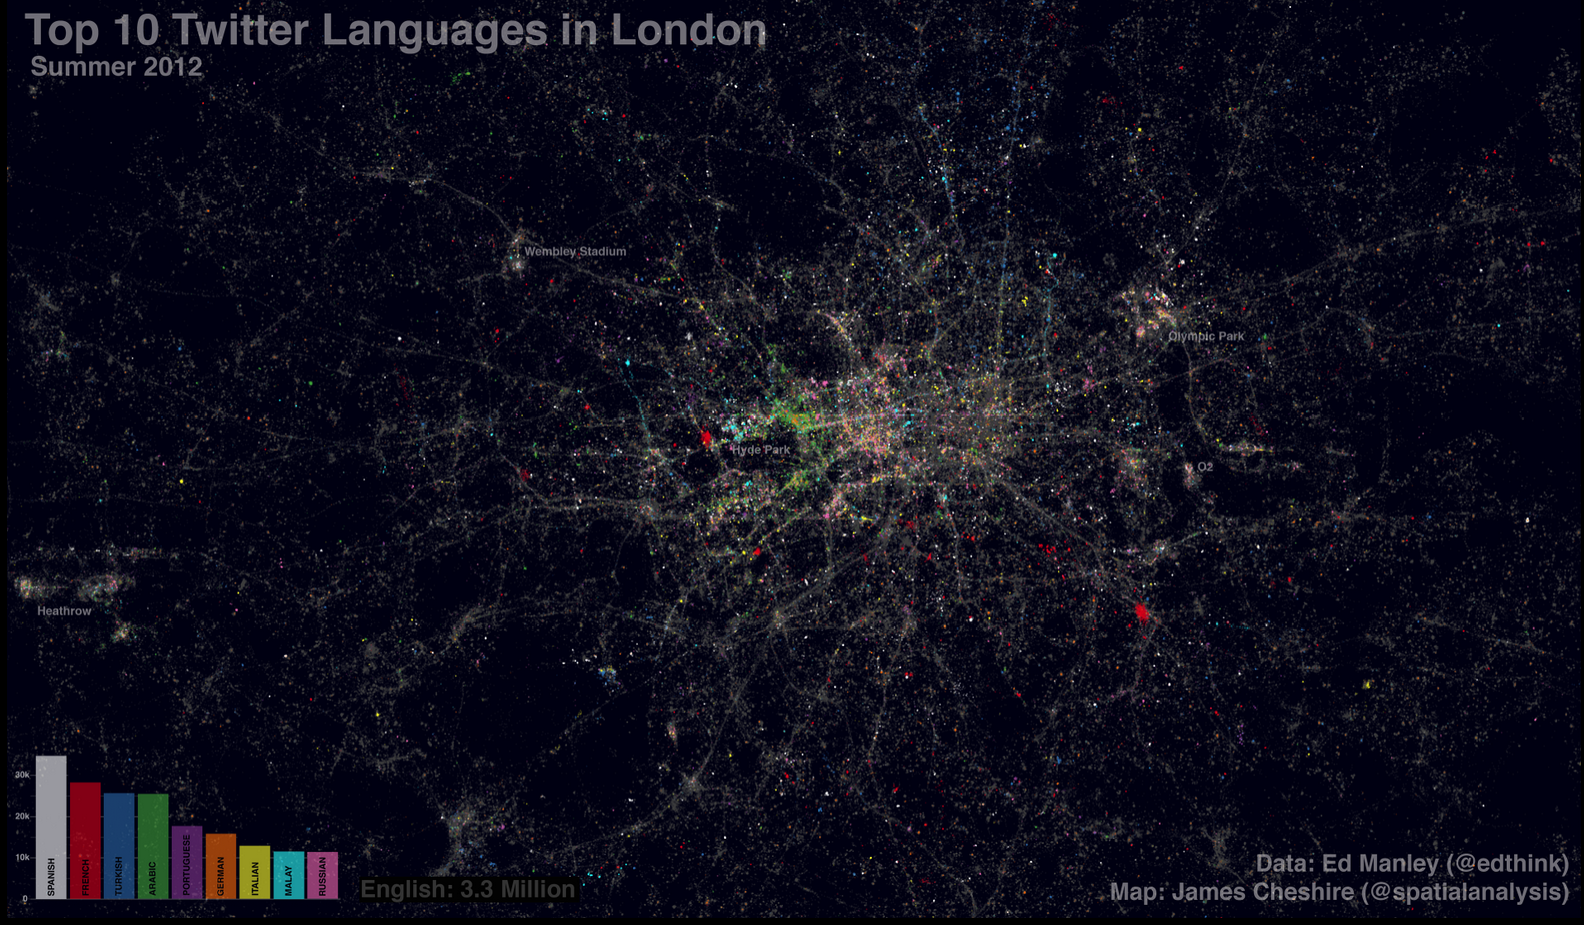
\includegraphics[width=\textwidth]{pix/twitter_lang_london.png}
\caption[Twitter Languages in London]{Twitter Languages in London\cite{Cheshire2012}}
\label{fig:twitter_london}
\end{figure}

These accumulations can be interpreted as geographical topics. \enquote*{A geographical topic is a spatially coherent meaningful theme. In other words, the words that are often close in space are clustered in a topic.}\cite{Yin2011} Geographical topic discovery has several use cases.\cite{Sizov2010} Companies offering free web-services can employ them very efficient because of their vast capacities and unfiltered access (if they have many active users).
\begin{description}
\item[Content organization] Modern cameras (especially mobile phone cameras) have the ability to save each photo with the location where it was taken. By using the location data the photos can be automatically categorized, or filtering when later searching for specific pictures of a landmark. Annotations and tags can be applied based on location,  direction and content of the photos.

\item[Search with spatial awareness]
Search engines can leverage additional spatial data, like GPS locations or keywords, to refine the search results. 

For example when searching for a restaurant with a mobile phone, the search application can either automatically commit the GPS data, or filter the results of the search engine based on it; without explicit knowledge of the user.

\item[Tag recommendation]% and exploration]
This use case is similar to the first example with photo annotations based on the location. Different specific locations can be recommended based on the given keywords.

For example when searching for the next holiday location and typing  \enquote{sun, beach, europe}, recommendations for further keywords could either be Nice (France), Crete (Greece) or Tenerife (Spain).

\item[Targeted advertisement]
Companies can optimize their strategies whether they should spend money on advertisement in regions where their product is already well known, or if they should rather advertise in other regions with similar geographic features, but less sales.
\end{description}
%
Besides these search, recommendation and exploration uses, geographic topics can also be used as early-warning system if timestamps are used. Various works explore these cases, mostly Twitter related for its active community and real time streaming API\cite{Vieweg2010, Mendoza2010, Hughes2009}.


\section{Problem Statement}
Using a dataset $D = \{d_1, \dots, d_n\}$ of geo-tagged documents $d_i = {text_i, location_i}$, and a cluster algorithm, meaningful geographic topics have to be found with a distance function based on a graph algorithm, which incorporates $text_i$ and $location_i$. The baseline compare function is composed of a naive linear combination of distance functions using $text_i$ and $location_i$ on vector representations of the data.

Extensive quantitative and qualitative evaluation of the results of these distance functions will be done done, using standard cluster evaluation measures with real world datasets. Evaluation includes the performances of the distance functions, as well as the performance of the evaluation measures in distinguishing between good and bad geographic topic results.

\vspace{.5em}
\noindent
As seen later in related works, evaluations are usually with rather small datasets, in contrast to the constant reminders of growing datasets. Datasets labelled with a ground truth (telling how the documents should be grouped) are evaluated using standard methods, but their datasets are small. If there are quantitative evaluations employed, on the small datasets, the comparison to different works is very hard to make.

Contributions of this thesis are the deployment of an extensible graph algorithm for finding geographical topics and its comparison to a naive baseline. And the consideration of cluster evaluation measures for quantitative evaluation of geographic topics with massive datasets containing more than one million points.

\vspace{.5em}
\noindent
The remaining thesis is structured as follows:

Chapter~\ref{chap:topics} introduces the general concepts of geographical topic models, clustering and lists the related works. Afterwards in chapter~\ref{chap:cluster} the used clustering algorithm is presented, and the used baseline distance function is motivated. Chapter~\ref{chap:graph} gives a general introduction to graphs and graph based algorithms, followed by a presentation of the graph-based approach by \textcite{Zhou2009} alongside some implementation adoptions. An explanation of the graph generation from the datasets concludes this chapter. Finally chapter~\ref{chap:eval} begins with a description of the different used evaluation metrics together with examples about their strengths and weaknesses. Subsequently the used datasets are introduced and the choice of parameters is discussed. The resulting comparison between the vector- and graph-based approaches with quantitative and qualitative evaluations leads directly to the conclusion of the thesis with a summery and future work in chapter~\ref{chap:future}.




%\section{Thesis Goals}
%Searching (and finding) such accumulations (clusters) among millions of points is called \emph{clustering}. Clustering is a common technique, with many different approaches, whose aim is to group similar objects together. Similarity is usually defined as distance, where smaller values indicate greater affinity.
%
%
%Geo-tagged data has a natural similarity measure among points, which is the distance $d_{location}$ between the locations from where the data has been transmitted. Clustering using this similarity measure can be interesting, but can be more interesting and meaningful if combined with other information. For example figure~\ref{fig:twitter_london} would be less than half as intriguing without the language information.
%
%This language information can be seen as a form of \emph{topic}. A topic is generally seen as a combination of words\,/\,sentences or other useful information describing or forming an abstract idea or general meaning. Using figure~\ref{fig:twitter_london} again, every tweet containing words or sentences have had their topic assigned as the recognized language of those words or sentences. It is clear that the process of finding such topics is heavily dependent on the used data and the use case for those topics.
%
%A simple form of topic detection is clustering the data points with a distance $d_{topic}$ based on processing the words or sentences contained in the data points. Every cluster can then seen as a topic, described by the contained words and their frequencies.
%
%Combining these two leads to \emph{geographical topic detection}. This task aims at providing useful regional topics.
%
%
%
%Using vector-based distance measures for text\,/\,topic distance $d_{topic}$ and geographical distance $d_{location}$, a combined distance $\alpha \, d_{topic} + \beta \, d_{location} = d_{combined}$ can be used to cluster both geographical and topical close objects, hopefully resulting in useful regional topics.
%
%\vspace{1em}
%\noindent
%Another approach is by performing abstractions. A graph can be a useful abstraction in working with objects having some sort of relationship with each other. A graph consists of nodes (objects), edges between those nodes (relationships) and attributes on either nodes or edges (features\,/\,weights). The affinity between objects in terms of text\,/\,topic distance and geographical distance will be represented by edges and weights.
%
%An example of a graph is a street map. Nodes are different cities, villages or other travelling targets. Edges are the streets connecting them, which represents the relationship of being able to travel from one point of interest to the next. Attributes are the names of the cities, or the speed limit of the streets. Defining the distance between two cities (nodes) can now be done based on the different streets (edges), for example the shortest\,/\,fastest route, the number of routes with maximal distance or travelling time and so on.
%
%For the task of identifying geographical topics a graph-based distance measure $d_{graph}$ will be used, which basically counts the number of possible routes between two nodes within a maximum length of these routes\cite{Zhou2009}. The higher the count the nearer\,/\,more similar the nodes are.
%
%
%
%
%\vspace{1em}
%\noindent
%This graph-based distance approach will be extensively compared to the above vector-based clustering with combined distances. In order to accomplish that, the clustering algorithm DBSCAN will be introduced in chapter~\ref{chap:cluster} together with the vector-based text and geographical distances.
%
%Chapter~\ref{chap:graph} explains the generation of the graphs from the datasets, followed by a presentation of the graph-based approach by \textcite{Zhou2009} alongside implementation adoptions.  
%
%Finally chapter~\ref{chap:eval} about the evaluation begins with describing the different used evaluation metrics and datasets. The resulting comparison between the vector- and graph-based approaches comes next, followed by the conclusion of the thesis with a summery and future work.
%
%\todo{Problem Statement}
%\todo{Contributions}

% !TeX program = lualatex
% !TeX root = main.tex

\chapter{Geographical Topic Discovery}
\emph{%
This chapter sets the background of geographic topic detection and employs the basic definitions of those. Related works and the Problem statement are described at the end of this chapter.
}\label{chap:topics}


\section{Background and definitions}
Data source for geographical topic discovery can be every web-service collecting geo-referenced data with access for developers and researchers. Popular ones are Twitter, Flicker, Open Street Map.

A geo-referenced dataset $D$ consists of different documents $\{d_1,\dots, d_n\}$. Each document $d$ has at least the following two \emph{attributes}:
\begin{description}
\item[text,] which is essentially a \enquote{bag of words}: a vector of different individual words or \emph{tags}.
\item[location,] which is a point $p \in \mathbb{R}^2$ determining a position on earth. $p$ is typically a GPS position, whose two parts are called \emph{longitude} and \emph{latitude}.
\end{description}
%
Other attributes are possible, like user identification, timestamp or user gender, but that depends on the used source. 

When using a vector-based model, each of those attributes are encoded in a vector $v^i_1, \dots, v^i_n$ for any given document $d_i$. Algorithms like the used distance measures then operate on these vectors. The vector-representation for the location is just the coordinates $lon, lat$. Text is represented by a vector whose length $m$ is the number of unique words in the dataset. Each word of these words is represented by a position in the vector. Each document then sets these positions to the number of occurrences in its text attribute. This model is also called bag-of-words, because it does not keep the positional information of the original text attribute. This means the original text attribute can not be deduced based on this vector. The distance functions used on the vector representations of location and text are described in section~\ref{sec:distance}.

Graphs are another way of symbolising the data. A graph $G = (V, E)$ consists of a set of \emph{nodes} $V$ and a list of \emph{edges} $E$ connecting different nodes. $v, w \in V$ and an edge $e_{v\,w} \in E$ connecting these nodes can have different properties, like weights or probabilities. Edges can have different directions, so that $e_{v\,w} \neq e_{w\,v}$. An example of a graph is a street map. Nodes are different cities, villages or other travelling targets. Edges are the streets connecting them, which represents the relationship of being able to travel from one point of interest to the next. Attributes are the names of the cities, or the speed limit of the streets. Defining the distance between two cities (nodes) can now be done based on the different streets (edges), for example the shortest\,/\,fastest route, the number of routes with maximal distance or travelling time and so on.

There is no common definition about what a \emph{geographical topic} is exactly, but the general idea is like: \enquote*{A geographical topic is a spatially coherent meaningful theme. In other words, the words that are often close in space are clustered in a topic.}\cite{Yin2011} A proper definition is usually coupled with a specific use case or a particular technique. Cluster analysis is used in this thesis to find geographical topics.

\emph{Cluster analysis} is the task of grouping a set of objects $\{o_1, \dots, o_n\}$ in such a way that objects in the same group are more similar to each other than to those in other groups. Those groups are called \emph{clusters}. The result of a clustering algorithm performing this analysis is a \emph{clustering}: a set of clusters $c_1, \dots, c_m$. Similarity is expressed as a distance function $f: o_i \times o_j \rightarrow \mathbb{R}$.

%Definition
\vspace{.5em}
\noindent
A geographic topic is defined in the following way. Given a 
\begin{itemize}
\item geo-referenced dataset $D=\{d_1,\dots, d_n\}$, 
\item a distance function $f(d_i, d_j)$, which utilises at least the document attributes $location$ and $text$, and 
\item a clustering algorithm: $D \times f \rightarrow c_1, \dots, c_m$, 
\end{itemize}
a \emph{geographic topic} is then represented by each cluster $c_i$.

\vspace{.5em}
\noindent
How well the clusters ${c1, \dots, c_m}$ are representing meaningful geographical topics is obviously controlled by those given parts.

Examples for geographic topics are cities or countries, events and festivals, countrysides like mountains and seas, and so forth. They are so different in meaning and space, that further disambiguation is helpful for understanding and comparing different types of and works about geographic topics. The following classification by \cite{Sengstock2011, Sengstock2012a} presents a good overview which fits for the most cases:
\begin{description}
\item[Global] Topics which have a very large spacial scale; they can be as large as the dataset itself. Other topics are usually covered by this.

Examples: countries and continents
%The spatial distribution of a feature being used equally likely by users all over geographic space is expected to follow a baseline distribution of the document collection. Such a feature is not informative to describe the semantics of geographic locations, except for the amount of user contribution. We assume the baseline distribution B to be the logged number of distinct users at a location l i . Then B(l i ) is the number of distinct users at l i . A feature with a distribution similar to B is expected to be a global feature.
%Global Feature: A global feature is distributed in the whole area of interest. A global feature is not distributed randomly (Poisson) but follows the density of the points in the dataset. This means that a global feature is also clustered. However, such a point pat- tern will be most similar to the point pattern of the complete dataset R.

\item[Landmark] This classification describes topics which are rather unique in the dataset and allows for labelling or describing a very specific place.

Examples: city and location names
%A feature might only be used around a single location l i (e.g., a city or place name). Such a feature allows to identify a location and acts as a descriptive label. However, such a feature will not allow us to discriminate between large proportions of geographic space, except between the location where the label occurs and the rest. We call a feature exhibiting such a property a landmark feature.
%A landmark feature describes a unique place on Earth, like a city or a place name. In this case, the point pattern shows a single cluster.

\item[Regional] Topics describing the environment. Landscapes and general appearance of this space.

Examples: forests, seas, mountains
%A feature might be used in a substantial part of geographic space. However, its usage might differ significantly from the baseline distribution B. Such a feature is expected to contain relevant geographic information for large parts of the geographic space, allowing us to compare locations based on their semantics. We call such a geographic feature a regional feature.
%Regional Feature: A regional feature occurs in a broad region on Earth. A regional feature might occur at several places on Earth, like the feature “forest”. In this case, the pattern is clustered within the radius of a typical region.

\item[Local] These topics are similar to landmark topics, but more general and not unique. They can appear everywhere and a rather focussed on a single spot. Events and festivals count here as well.

Examples: supermarkets, restaurants, conferences

%A local feature occurs locally at several places on Earth, like a feature occurring mainly in cities. The point pattern is highly clustered within the radius of a city area.
\end{description}
%
These descriptions and examples are very general to be adaptable to different use cases and dataset scales. The scale (or scope) is here very important. For a dataset with points all over the world, factories from different companies can be classified as local topics, while a \enquote{named} forest can be a landmark. Using a dataset which is completely covered by this forest, a factory can be a landmark, and this very forest is a regional or even global topic.

% use cases


\section{Related Work}
The related work is focussed on how geographic topics can be modelled, how the results then are evaluated and how graphs algorithms can be used on this task.

The following contributions use generative models to find geographic topics. This means, instead of trying to calculate the conditional probability distribution of a topic given a tweet $p(topic | tweet)$, the joint probability $p(tweet, topic)$ is modelled. This joint probability can be used to \emph{generate} likely ($topic$, $tweet$)-pairs, thus generative model. Using an inference algorithm like naive Bayes or expectation maximisation, the joint probabilities can be transformed to conditional probabilities and then used to classify tweets into topics.

\begin{itemize}
\item \textcite{Sizov2010} proposes GeoFolk. This model aims to construct better algorithms for content management, retrieval, and sharing in social media. GeoFolk assumes that each topic generates latitude and longitude from two topic-specific Gaussian distributions. The approach is based on multi-modal Bayesian models which allows integration of spatial semantics of social media in a well-formed, probabilistic manner. This work uses Gibbs Sampling for inference.
 
Evaluation is done with a Flickr dataset containing only resources from the greater London area (28\,770 points). Results are compared to LDA (Latent Dirichlet allocation, also a Bayesian model) with Deviance Information Criterion (DIC), which considers  the corresponding model complexity and trade-offs between the fit of the data to the model. Manually labelled data was also used to compare accuracy in classification and recommendation tasks. 

\item \textcite{Yin2011} describes three ways of modelling geographical topics: a location-driven, a text-driven model (which are later used as a comparison baseline) and a unified model called LGTA (Latent Geographical Topic Analysis). The idea here is the assumption of a set of regions who generates the topics (instead of documents generating the topics). Two words belonging to the same region are close in space, and should be more likely to be clustered into the same geographic topic.

%Yin et al. [17]: Their method is essentially to have
%a global set of topics shared across all latent regions.
%There is no regional language models in the model.
%Besides, no user level preferences are learned in the
%model. The prediction is done by two steps: 1) choos-
%ing the region index that can maximize the test tweet
%likelihood, and 2) use the mean location of the region
%as the predicted location. We re-implemented their
%method in our work. This method is denoted as Base-
%line.
%The inference is done by MAP-style EM. 

%In this paper, we are interested in two questions: (1) how to
%discover different topics of interests that are coherent in geo-
%graphical regions? (2) how to compare several topics across
%different geographical locations? 

%To answer these questions,
%this paper proposes and compares three ways of modeling ge-
%ographical topics: location-driven model, text-driven model,
%and a novel joint model called LGTA (Latent Geographical
%Topic Analysis) that combines location and text. 

%To make
%a fair comparison, we collect several representative datasets
%from Flickr website including Landscape, Activity, Manhat-
%tan, National park, Festival, Car, and Food. The results
%show that the first two methods work in some datasets but
%fail in others. LGTA works well in all these datasets at
%not only finding regions of interests but also providing ef-
%fective comparisons of the topics across different locations.
%The results confirm our hypothesis that the geographical
%distributions can help modeling topics, while topics provide
%important cues to group different geographical regions.

Evaluation is done with different representative datasets from Flickr covering several topics: Landscape, Activity, Manhattan, National Park, Festival, Car and Food, each containing between 1\,751 and 151\,747 points. Comparison baseline techniques are the presented location- and text-driven models, as well as GeoFolk\cite{Sizov2010}. The models were evaluated using perplexity, which calculates how well a probability model $q$ predicts an unknown model $p$ based on test samples drawn from $p$. Results were also discussed based on expected amounts of found topics in the respective datasets and their visualisations.
%  discussion and qualitative analysis

\item \textcite{Hong2012} incorporates the information by which user a tweet was sent. The generative process is modelled on the assumptions, that words in a tweet are dependent on the location as well as the topic, which leads to different discussed topics in different locations, and finally that users only have distinct regions, where they live, and thus from where they sent tweets.

% 1) How is information created and shared
%across geographical locations, 2) How do spatial and linguis-
%tic characteristics of people vary across regions, and 3) How
%to model human mobility. 

% In this paper we focus on
%Twitter and present an algorithm by modeling diversity in
%tweets based on topical diversity, geographical diversity, and
%an interest distribution of the user. Furthermore, we take
%the Markovian nature of a user’s location into account. Our
%model exploits sparse factorial coding of the attributes, thus
%allowing us to deal with a large and diverse set of covariates
%efficiently. 

%We show high accuracy in location estimation based on our
%model. Moreover, the algorithm identifies interesting topics
%based on location and language.

Evaluation is based on a Twitter dataset with 573\,203 distinct tweets from 10\,000 users between January 2011 and May 2011, and a dataset from \url{http://www.ark.cs.cmu.edu/GeoText/} with 377\,616 messages from 9\,475 users. Both datasets are geo-tagged and locations are approximately within the United States. Comparison is done amongst others with \cite{Yin2011}, by predicting the location for every tweet and then calculating the distance to its real location.

%The size of the dataset is significantly larger than the ones used in some similar studies (e.g, [7, 17]).
\end{itemize}
%
The following are no generative models.

\begin{itemize}
\item \textcite{Sengstock2012a} examine the use of dimensionality reduction techniques PCA, ICA and Sparse PCA (SPCA) on a matrix of high-dimensional multivariate signals of geographic semantics in order to extract meaningful geographic features. % which are processed feature-vectors to represent the characteristics of a geographic location.
Normalization of the data is used to find specifically landmark, global, ... topics.

%In this work we present a framework for the unsupervised
%extraction of latent geographic features from georeferenced
%social media. 

%A geographic feature represents a semantic
%dimension of a location and can be seen as a sensor that
%measures a signal of geographic semantics. Our goal is to
%extract a small number of informative geographic features
%from social media, to describe and explore geographic space,
%and for subsequent spatial analysis, e.g., in market research.

%We propose a framework that, first, transforms the unstruc-
%tured and noisy geographic information in social media into
%a high-dimensional multivariate signal of geographic seman-
%tics. Then, we use dimensionality reduction to extract la-
%tent geographic features. 

%We conduct experiments using two
%large-scale Flickr data sets covering the LA area and the
%US. We show that dimensionality reduction techniques ex-
%tracting sparse latent features find dimensions with higher
%informational value. 

%In addition, we show that prior nor-
%malization can be used as a parameter in the exploration
%process to extract features representing different geographic
%characteristics, that is, landmarks, regional phenomena, or
%global phenomena.
Evaluation is done by using two Flickr datasets, covering LA with 245\,312 points, and the US with 5\,976\,689 points. PCA, ICA and SPCA are then qualitatively compared by discussing three selected geographic topics.


\item \textcite{Yen2005} proposes the use of a distance metric called the Euclidian Commute Time (ECT) distance, which is based on a random walk model. The graph is derived from the data by connecting every node to its k nearest neighbours. This distance can then be used in every applicable clustering algorithm.

Evaluation is done with synthetic datasets against normal euclidean distance. Results are visually examined and compared.

\item \textcite{Cao2010} uses the graph concept to extract meaningful semantic locations (points of interest) from GPS data showing the movement of cars in daily use. This is accomplished by building a layered graph of two connected sub-graphs: a location-location graph, representing visits\,/\,stops on a trip and a user-location graph standing for users visiting certain locations. Clustering is used to group visit points. Then a combination of PageRank, HITS (both using a random walk distance), is used to find semantic locations.

Evaluation is done on three subsets of the whole dataset obtained by 119 cars and originally 0.1 billion GPS records, distilled to 76\,139 stay points. The three subsets contain 352, and two times 1\,508 locations. Those locations where than manually annotated in order to use entropy, purity, and normalized mutual information (NMI) to evaluate the clustering. The smaller the entropy, the better a clustering method performs. For the other two measures, the larger, the better. Location significance ranking were evaluated with Mean Average Precision (MAP), Precision@n, and nDCG (normalized Discounted Cumulative Gain).
\end{itemize}

% Problem statement


% !TeX program = lualatex
% !TeX root = main.tex

\chapter{Clustering and combined distances}
\emph{%
This chapter covers the basics of clustering. It first describes the used clustering algorithm DBSCAN, followed by the distance metrics for geographical distance and text distance. At last the combined distance metric is presented.
}\label{chap:cluster}

\section{Cluster analysis}
As introduced in chapter~\ref{chap:topics}, \emph{cluster analysis} is the task of grouping a set of objects $\{o_1, \dots, o_n\}$ based on similarity, which is expressed as a distance function $f: o_i \times o_j \rightarrow \mathbb{R}$. There are many different clustering algorithms\cite{Berkhin2006}, each with there own problems and advantages. Two often used concepts are hierarchical clustering, and k-means.

\subsubsection*{Hierarchical clustering}
Hierarchical clustering builds a hierarchy,\,/\,tree of documents called dendrogram. The cluster set can be retrieved for example by choosing a tree level; then all child nodes which have the same parent at this level are together in a cluster. The dendrogram can be computed in two ways: 
    
Agglomerative, which starts with each document as its own cluster, and then joins them successively (\enquote{bottom up} approach). Or divisive, which starts with one giant cluster, and then performs splits recursively, until every document is alone (\emph{top down} approach).

The definition of a distance between the clusters, based on which all joining\,/\,splitting happens, is called link criterion. There are many different ones; two obvious examples are complete linkage clustering $\max \{f(a,b): a \in A, b \in B\}$ and single-linkage clustering $\min \{f(a,b): a \in A, b \in B\}$. 

A great problem with using hierarchical clustering is the complexity of at least $O(n^2)$, especially considering the big datasets used in this thesis.

\subsubsection*{k-means}
k-means clusters objects into $n$ clusters. At the beginning, $n$ points are chosen as initial cluster centroids. Then each point is being assigned to the nearest cluster center. After that new cluster centroids are calculated, usually the mean of all points assigned to it. Point assignment and center recalculation is done until the centroids are stable.

The k-means algorithm is relatively simple and easy to adopt to new domains and tasks, which explains its popularity. Finding a global optimal solution is considered NP-hard, but there are approximations with polynomial complexity, or solutions for \enquote{good enough} results by carefully choosing the initial cluster centroids.

Problems with k-means are the initial choice of the number of clusters and, depending on the distance function, the weakness in finding arbitrary shaped clusters.

\vspace{1em}
\noindent
This leads directly to the used clustering algorithm, which does not have the problems of the two ones described above.

\section{DBSCAN}
DBSCAN (density-based spatial clustering of applications with noise) by \textcite{Ester1996} is a density-based clustering algorithm. It is able to detect arbitrary shaped clusters and does not need the number of clusters beforehand. It performs also well with a complexity of $O(n \log n)$, which makes it usable for big data sets, and it has a notion of noise; of points which are so different they belong to no cluster.

Density describes the amount of elements in a given area. DBSCAN defines this as the $\epsilon$- or $eps$-neighbourhood $N_{eps}(p)$ of a point $p$, which are all points $q$ with distance $d(p, q)$ smaller $eps$.
%
\begin{align*}
N_{eps}(p) &= {q \in D | d(p,q) \leq eps}
\end{align*}
%
Furthermore DBSCAN differentiates between two kinds of points: 
%
\begin{align*}
|N_{eps}(p)| \geq minPts &\rightarrow core\\
else &\rightarrow border
\end{align*}
%
$core$ points have at least $minPts$ in their $eps$ neighbourhood, $border$ points have less.

Density as the amount of elements in a given area is naturally described by $N_{eps}$ and $minPts$. These dense neighbourhoods of core points are then connected through their density. A point $p$ is directly density reachable from $q$, if $p \in N_{eps}(q)$ and $q$ is $core$ point. Directly density reachability is asymmetric if one of the two points is a $border$ point.

Extending on directly density reachability is the definition of density reachability. A point $p$ is density reachable from a point $q$, if there is a path of points $p, p_1, \dots, p_n, q$, so that $p_{i+1}$ is directly density reachable from $p_i$. This is again asymmetric, if one of the two points is a $border$ point.

Because two $border$ points can not density reach each other, the notion of density connectivity is introduced, which is symmetric. Two points $q$ and $p$ are density connected, if there is a third point $k$ that can reach both $q$ and $p$ through density reachability. Clusters and noise are now defined based on density connectivity. 

A cluster $c$ is a subset of documents of a dataset $D$ with regard to $eps$ and $minPts$, so that for all $core$ points $p, q \in c$ are density reachable to each other, and all $border$ points are density connected to $core$ points. If $c_1, \dots, c_n$ are all clusters of $D$ (always regarding $eps$ and $minPts$), then $noise$ are all those points not belonging to any cluster.

Every cluster has a size of at least $minPts$. DBSCAN has stable results regarding $core$ points; they are always in the same cluster, regardless of the order of processing, because they are always density reachable. $border$ points can change their affiliation of a cluster, because they could be reached by different $core$ points, who could belong to different cluster.

\newpage
\subsection{Algorithm}
As previously seen, DBSCAN requires the following two parameters:

\begin{enumerate}
\item $eps$ (eps), which defines the minimum distance of $p$ to all points in $N_{eps}(p)$, and
\item $minPts$, which defines the minimum number of points needed inside $N_{eps}(p)$ for $p$ to be a core point.
\end{enumerate}

A pseudo code of the algorithm can be found in listing~\ref{dbscan}. DBSCAN starts at an unvisited random point $p$ and checks if $|N_{eps}(p)| \geq minPts$. If this requirement is not met, $p$ will be marked as noise. $p$ could later be reached by another point and thus clustered being a border point. If $|N_{eps}(p)| \geq minPts$ is true a new cluster $C$ is created. 

Now every point $q$ in $N_{eps}(p)$ is added to the cluster $C$ (if not already in another cluster as a border point). Iteratively the size of every $N_{eps}(q)$ is checked and points added to $N$ for further investigation until $N$ is empty.

At last the circle starts again with another random, unvisited point, until all points are visited.

\begin{algorithm}[tb]
\caption{DBSCAN algorithm}\label{dbscan}
\begin{algorithmic}[1]
\Function{DBSCAN}{D, $eps$, $MinPts$}
\ForAll{p $\in$ D, p \textbf{not marked as} VISITED}
	\State \textbf{mark} p \textbf{as} VISITED
	\State N \gets D.regionQuery(P, $eps$)
	\If{\Call{sizeof}{N} $\geq MinPts$}
		\State C \gets next cluster
		\State \Call{expandCluster}{p, N, C, $eps$, $MinPts$}
	\Else		
		\State \textbf{mark} p \textbf{as} NOISE
	\EndIf
\EndFor
\EndFunction
\Statex
\Function{expandCluster}{p, N, C, $eps$, $MinPts$}
\State \textbf{add} p \textbf{to} cluster C
\ForAll{q $\in$ N, q \textbf{not marked as} VISITED}
	\State \textbf{mark} q \textbf{as} VISITED
	\State M \gets \Call{regionQuery}{q, $eps$}
	\If{\Call{sizeof}{M} $\geq MinPts$}
		\State N \gets N $\cup$ M
	\EndIf
	\If{q is not yet member of any cluster}
		\State \textbf{add} q \textbf{to} cluster C
	\EndIf
\EndFor
\EndFunction
\Statex
\Function{regionQuery}{p, $eps$}
\State \Return all points within $N_{eps}(\text{p})$
\EndFunction
\end{algorithmic}
\end{algorithm}

The algorithm performs basically a $regionQuery$ for every point in the dataset in order to get all $eps$ neighbourhoods. Hence the complexity of DBSCAN depends on the complexity for this $regionQuery$: $O(n \, \, O(regionQuery))$. A very simple $regionQuery$ can be a linear search over all other points, resulting in an overall complexity of $O(n^2)$, which is effectively a distance matrix. Such a distance matrix can be precomputed for subsequent execution on the same dataset, but this would require $O(n^2)$ memory. Usually a better strategy involves the usage of an appropriate index structure, for example R-trees or kd-trees, which work very well for spatial data. Most of these index structures have an average neighbourhood search complexity of $O(\log n)$, with leads to an overall average complexity of $O(n \log n)$ for DBSCAN.

Datasets with very various densities can be problematic, because the two parameters $eps$ and $MinPts$ only describe one density threshold. Hence DBSCAN is unable to detect a cluster within another cluster with different density, as long as both are denser than the threshold. Also the used distance\,/\,neighbourhood function must be chosen carefully; the so called \enquote{curse of dimensionality} can render any $eps$\,/\,$MinPts$ combination useless due to high dimensional data with an unfitting distance function.

DBSCAN does not require the number of cluster beforehand. This is especially useful if there is no viable visualization or there is no clue for guessing. Arbitrary shaped clusters can be found, and points have not to be clustered at all, if they are too different (noise). Building clusters depends only on the distances between points; in fact, they depend only on the $eps$-neighbourhood queries, which enables the usage of a wide variety of data and distance\,/\,neighbourhood functions.


\section{Distance Metrics}\label{sec:distance}
Besides the choice of the two parameters for DBSCAN, the underlying distance function is of great importance. This distance function has to follow some rules in order to be useful in DBSCAN. It has to obey the following first two rules from the definition of a metric (all rules given for completeness, and because most useful distance functions are metrics after all).

A metric on a set $X$ is a function (called the distance function or simply distance) $d : X × X → R$. For all $x, y, z$ in $X$, this function is required to satisfy the following conditions:
\begin{enumerate}
\item $d(x, y) \geq 0$ (non-negativity)%, or separation axiom)
\item $d(x, y) = d(y, x)$ (symmetry)
\item $d(x, y) = 0$ if and only if $x = y$ %(identity of indiscernibles, or coincidence axiom)
\item $d(x, z) \leq d(x, y) + d(y, z)$ (triangle inequality)%subadditivity
\end{enumerate}

%\subsection{Time distance}
%The distance between two timestamps $t_1$ and $t_2$ is the time passed between those two events; the timespan between them:
%\begin{align*}
%d^{time}_{12} = |t_1 - t_2|
%\end{align*}
%The interval of $d^{time}$ is $[0, t_{max}-t_{min}]$.

\subsection{Text distance}
There are many different distance metrics to measure the (dis)similarity between texts respectively documents\cite{Huang2008}. Depending on the lengths of the text and the additional tasks upon them (searching, ranking), it is important to use an appropriate metric.

The distance metric used in this thesis for texts is the Jaccard distance\cite{Manning2009} on top of bigrams of the texts, which has been effectively used for clustering text\cite{Huang2008}. A bigram is the set of all adjacent two-letter fragments of a text. For example the word $distance$ has the following bigram: $(di, is, st, ta, an, nc, ce)$. The Jaccard index $J$ is defined as the size of the intersection divided by the size of the union of two bigrams $A$ and $B$. This measures the similarity of the two sets. The Jaccard distance $d_{text}$ is then calculated by subtraction of $J$ from $1$:
%
\enlargethispage{\baselineskip}
\begin{align}
J(A, B) &= \frac{|A \cap B|}{|A \cup B|}\notag\\
d_{text}(A, B) &= 1 - J(A, B) = \frac{|A \cup B| - |A \cap B|}{|A \cup B|}
\end{align}
The interval of $d_{text}$ is $[0, 1]$.

\subsubsection{Example}
The text distance between the words \emph{distance} and \emph{maintenance} has to be calculated. The sets $A$ and $B$ contain the bigrams:
\begin{align*}
A &= di, is, st, ta, an, nc, ce\\
B &= ma, ai, in, nt, te, en, na, an, nc, ce
\end{align*}
%
The intersection and union of $A$ and $B$ is as follows
\begin{align*}
|A \cap B| &= |an, nc, ce| = 3\\ %intersection
|A \cup B| &= |di, is, st, ta, ma, ai, in, nt, te, en, na, an, nc, ce| = 14 %union
\end{align*}
%
which leads to the final distance
\begin{align*}
d_{text} &= 1 - \frac{3}{14} \approx 0.786
\end{align*}

\subsection{Location distance}
The given GPS data (Latitude ($lat$)\,/\,Longitude($lon$)-pairs) are locations on the earth; positions on top of a (rather non-uniform) ellipsoid. The optimal way of computing the distance between two points would be in calculating the distance on top of this ellipsoid (great-circle distance).

But this is time-consuming and ugly to handle. Another way is to project the coordinates onto a plane and calculate an approximation with basic trigonometry and euclidean distances. This can be done thinking of the center of the earth as one corner of a triangle, and the two locations (whose distance from one another is wanted) as the other two corners, resulting in the following formula, which is sometimes called planar projection:

\begin{align*}
x &= (A_{lon} - B_{lon}) * cos(\frac{A_{lat} + B_{lat}}{2})\\
y &= (A_{lat} - B_{lat})\\
d &= R \, \frac{\pi}{180} \, \sqrt{x^2 + y^2}
\end{align*}
%
$R$ is \enquote{the} radius of the earth, which is 6373~km in this thesis. The factor $cos(\frac{A_{lat} + B_{lat}}{2})$ is used to correct the wide for one longitude degree, which \enquote{grows tighter} the nearer it is to the poles. This factor will be omitted for practical reasons (usage of a spatial index for fast neighbour queries), as well as $R$ and $\frac{pi}{180}$, which are not needed for just comparing distances.

\begin{align}
d_{loc}(A, B) &= \sqrt{(A_{lat} - B_{lat})² + (A_{lon} - B_{lon})²}
\end{align}
%
This euclidean distance is good enough for comparing distances. For example the great-circle distance between Berlin ($lat$: 52.66, $lon$: 13.51) and Bonn ($lat$: 50.74, $lon$: 7.10) is 739.52~km, while the euclidean distance is 6.69° or 744.26~km.

%\todo{comparison great-circle vs euclidean}

%>>> from pyproj import Geod
%>>> g = Geod(ellps='WGS84')
%>>> g.inv(52.655561,13.507462, 50.739932,7.10392)
%(-163.31731230887556, 16.339412526021903, 738694.1895019277)
%Berlin to Bonn
%great-circle distance 738.69~km
%>>> from math import sqrt
%>>> sqrt(pow((52.655561- 50.739932),2) + pow((13.5 - 7.10392),2))
%6.676786190379395
%>>> sqrt(pow((52.655561- 50.739932),2) + pow((13.5 - 7.10392),2)) * 0.017453292519943295769236907684886 * 6372797.560856
%742634.2238470017
%euclidean 742.63~km

%\begin{wrapfigure}{r}{0.40\textwidth}
%  \begin{center}
%    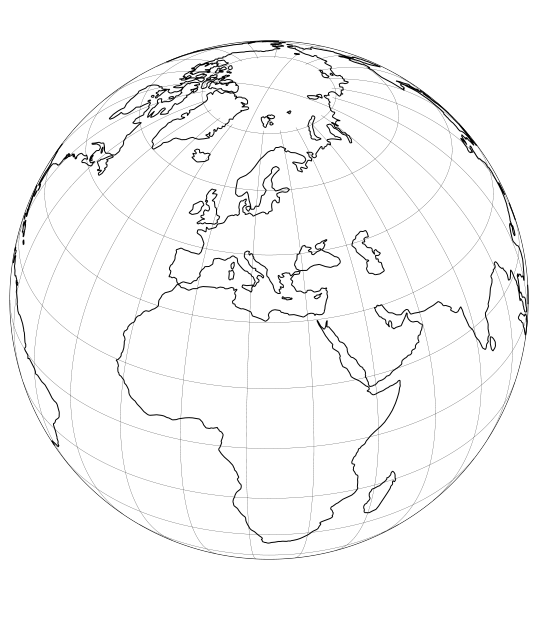
\includegraphics[width=0.38\textwidth]{pix/map_projection}
%  \end{center}
%  \caption{Globe with longitude and latitude lines\protect\footnotemark}
%\end{wrapfigure}

%\footnotetext{\url{http://kartograph.org/showcase/projections}}Locations are usually given in longitude\,/\,latitude-coordinates. This coordinate system divides the earth horizontally in 180 equal parts called latitude, which are parallel to each other. The north pole is 90°, the equator 0° and the south pole -90°.

%Longitude are called the 360 parts slicing the earth vertically. Those slices are not parallel; they start each at the north pole and end at the south pole.

%The earth is a rather non-uniform ellipsoid, hence each distance between two points is no straight line, but a path on a sphere at best. Distances on the surface of a sphere are called great-circle distances. Using euclidean distance is therefore prone to be more unprecise the greater the two points are afar and the greater the latitude gets.

%There are now three options depending the location distance measure:
%\begin{enumerate}
%\item Great-circle distance: precise, but slow to compute and no index-support.
%\item Euclidean distance: very fast to compute and index-support, but very inaccurate.
%\item Combination of both: use unprecise euclidean for nearest neighbour queries to reduce the possible candidates, the calculate the accurate distances with a great-circle distance.
%\item (alternative: dimension reduction for a projection of lat\,/\,lon to euclidean distances while preserving the distances)
%\end{enumerate}
 
%\section{Definitions}
%\begin{tabular}{ll}
%$d^n_{ij}$ & distance of type $n$ from $i$ to $j$\\
%\end{tabular}

\subsection{Combining the distance metrics}
After introducing the two fundamental distance metrics for text and location distances, they are joined in a linear combination in the form $\alpha \, d_{loc} + \beta \, d_{text} = d_{com}$. Of course, additional distance metrics could also be joined in the same linear fashion.

$\alpha$ and $\beta$ could be simple weights, but because the intervals of the metrics are different, they should also incorporate a way to align the distances. Thus, $\alpha$ and $\beta$ each consist of a weight $w$ and a normalisation factor $eps$. 

\begin{align}
d_{com} &= \alpha \,\, d_{loc} + \beta \,\, d_{text}\notag\\
d_{com} &= \frac{w_{loc}}{eps_{loc}} \, d_{loc} + \frac{w_{text}}{eps_{text}} \, d_{text}\\
\sum w &= 1 \notag
\end{align}
%
The normalization factor is called $eps$, because it has the same effect as the DBSCAN parameter $eps$, if one weight is set to 1 as well as DBSCAN $eps$:
\begin{align*}
1 &= \frac{1}{eps_{loc}} \, d_{loc} + \frac{0}{eps_{text}} \, d_{text}\\
&= \frac{1}{eps_{loc}} \, d_{loc}\\
d_{loc} &= eps_{loc}
\end{align*}
%
With this natural relation of these values, it is easy to understand the meaning of the normalization and finding usable values is much easier.

% !TeX program = lualatex
% !TeX root = main.tex

\chapter{Graph distance and generation}
\emph{%
This chapter begins with general use cases of graphs. The graph-based distance metric is then described together, as well as some adaptations. The chapter concludes with a discussion about the creation of a graph based on points in space.
}\label{chap:graph}

\section{Introduction}
Graphs $G = (V, E)$ were introduced in chapter~\ref{chap:topics} as a set of nodes $V$ and a list of edges $E$. Edges can have different directions, so that $(v_i, v_j), (v_j, v_i) \in E$, but $(v_i, v_j) \neq (v_j, v_i)$. The same applies to edge weights $w_{i\,j} \neq w_{j\,i}$. Weights are also denoted as $w_{v_i \, v_j}$. A path $\tau: v_i \leadsto v_j$ is a sequence of edges which connects two nodes $v_i$ and $v_j$ (similar concept as density reachability).

%Königsberger Brücken
The first usage of graphs in analysing a problem is thought to be in the famous paper by Leonhard Euler about the Seven Bridges of Königsberg from 1736. The problem was, if it is possible to cross the river Pregolya using all seven bridges of Königsberg once. He proved the impossibility of this task.

%Einsatzbereiche
Today, graph theory is an indispensable tool for logistical optimisation and planning, for example the (time-\,/\,cost-) optimal way of distributing goods with $m$ transporters to $n$ customers. Calculating the shortest or less time consuming way between two locations in a route guidance system is done with graphs. Popular social networks or network-like services embody a graph-like structure (relationship between people) and can therefore be analysed via graphs. Facebooks Graph Search%
\footnote{\url{https://www.facebook.com/about/graphsearch}}%
 and Open Graph framework%
 \footnote{\url{https://developers.facebook.com/docs/opengraph/overview/}}%
 emphasises this with their names.
But there are many other areas of application for graph theory and graph algorithms.

\vspace{3em}

%Darstellung, Speicher
Typical ways of storing graphs in memory are either
\begin{description}
\item[adjacency lists,] where each node has a list of his adjacent nodes and the corresponding weight, or
\item[adjacency matrices,] where each matrix entry $m_{i\,j}$ stands for an edge from node $i$ to node $j$, its value the corresponding weight of the edge.
\end{description}
%
The data structure choice depends, as always, on memory constraints and algorithm design using the graph. Figure~\ref{fig:graphexamples} shows a visualisation of a simple graph accompanied by its representation as adjacency list and matrix.

\begin{figure}[h]
%\centering
	\begin{subfigure}[b]{0.25\textwidth}
		\centering
		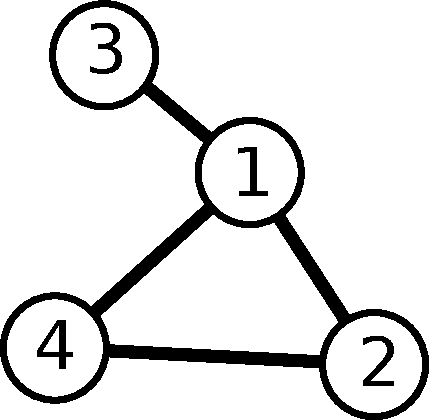
\includegraphics[width=\textwidth]{pix/simple_graph.pdf}
		\caption{Simple graph}
		%\label{fig:gull}
	\end{subfigure}
	\hfill
	\begin{subfigure}[b]{0.25\textwidth}
		\raggedright
		\qquad \begin{description} \itemsep -0.5em
			\item[1:] 2, 3, 4
			\item[2:] 1, 4
			\item[3:] 1
			\item[4:] 1, 2
		\end{description}
		\caption{Adjacency list}
		%\label{fig:gull}
	\end{subfigure}
	\hfill
	\begin{subfigure}[b]{0.25\textwidth}
		\centering
		$\begin{matrix}
			0&1&1&1\\ 1&0&0&1 \\ 1&0&0&0 \\ 1&1&0&0
		\end{matrix}$
		\caption{Adjacency matrix}
		%\label{fig:gull}
	\end{subfigure}
	%\hfill
\caption{Graph representation examples}\label{fig:graphexamples}
\end{figure}

\section{Clustering with graphs}
There are two basic concepts in how to cluster a dataset with the aid of a graph:
\begin{itemize}
\item Direct clustering with the graph structure, and
\item Deriving of features based on the graph, then clustering based on those features.
\end{itemize}
%
The main difference is the sort of clustering algorithm that can be used. Direct clustering requires a graph algorithm whose results are the final clusters. Using feature clustering is indirect, but every possible clustering algorithm can be used, if the derived features (for example a distance) are compatible. A few direct clustering approaches are now presented, to show some possibilities of graph algorithms, to better understand and compare to the feature derivation clustering used in this thesis.

\begin{description}
\item[Single link edge length] One of the simplest ways to directly cluster a graph based on its structure is to use agglomerative hierarchical clustering with single link edge length. This means that in each iteration the nodes connected by the edge with the lowest edge weights are joined in the tree, until all nodes are in one cluster.

\item[Minimum Spanning Trees]
A minimum spanning tree (MST) of a graph is a set of edges with accumulated minimum edge weight, so that every node can reach every other node through a path over those edges. Now whenever an edge is removed, this tree splits in two distinct trees without connection between them, also called connected components. Edge removal can then be iteratively applied until there are enough clusters, or until some other criterion is fulfilled. Selection of the edge to be removed can for example be based on the weight of the edge (remove edge with the highest weight), or a combination of edge length and cluster size like in~\cite{Muller2012}.

%subsection*{Normalized Cut}
\item[Normalized Cut]
Another way are normalized cuts, which seem to be often used in tasks involving image segregation, like in \cite{Shi2000}. The edge weights of an \enquote{image graph} are based on the differences between each pixel. Either every pixel connects to all other pixels in the whole picture, or (more often) every pixel connects to all adjacent pixels. The clustering idea is similar to minimum spanning trees: split the graph in two connected components based on the value of the cut, which equals the sum of the weights of the removed edges. This produces quite good results, but is prone to cut small, isolated groups of nodes in the graph. Thus the value of the normalized cuts is based on the sum of the removed edges versus the sum of the untouched edges. Cuts with minimum value are optimal and lead to more stable partitions.
\end{description}
%
The graph algorithm used for clustering in this paper yields distances between the nodes, which then are used in DBSCAN for clustering.

\section{Distances based on structural and attribute similarities}
The algorithm \emph{SA-cluster} described in the paper \enquote{Graph clustering based on structural\,/\,attribute similarities} by \textcite{Zhou2009} is based on the idea, that nodes close to each other should have many different paths between them. The examples from the previous section only utilise the structure of the graph, but no additional information from the nodes. Very different attributes like timestamps, gender, color, ..., or in this case text, can be further used to determine the closeness of nodes, and thus give better clusters. SA-cluster uses the graph structure and enhances it with the provided attributes to calculate node similarities. The paper also describes a way of automatically adjust the influence of different attributes based on their contribution the the clustering. Because only $text$ is used, there is no need to use it here.

%section~\ref{sec:graph_generation}

%The algorithm operates on a graph whose nodes have attributes: $G = (V, E, \Lambda)$. The only attribute used in this thesis is $text$, but more are possible. 

Figure~\ref{fig:sa} shows a graph with five nodes consisting of two subgraphs with text attributes. The similarity between node 1 and node 4 or node 5 would be $0$, because there is no path between them. But they have the exact same text attribute values, so they should have some similarity. The idea now is to generate additional paths between nodes who have matching attribute values. This is done by creating additional nodes for every possible attribute value, whose edges then connect to nodes having this value. These additional nodes $N_a$ and edges $E_a$ are called \emph{augmented} nodes\,/\,edges, the graph they create $G_a = (N_a, E_a)$ accordingly augmented graph, and the algorithm operates on the unified graph $G \cup G_a$. All following mentions of nodes, edges, and the graph in general are assumed to mean the unified case.
%
\begin{figure}[b]
\centering
	\begin{subfigure}[b]{0.40\textwidth}
		\centering
		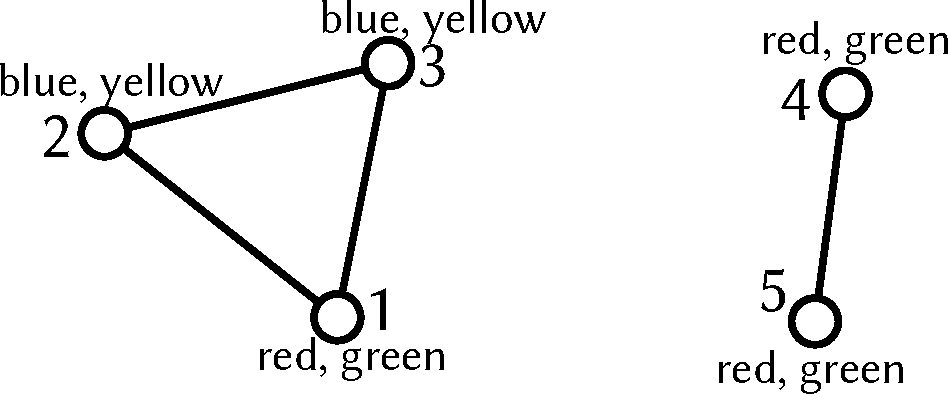
\includegraphics[width=\textwidth]{pix/SA1.pdf}
		%\caption{Simple graph}
		%\label{fig:gull}
	\end{subfigure}
	\hfill
	\begin{subfigure}[b]{0.05\textwidth}
	\centering	
	$$\Rightarrow$$\\
	\hspace*{\fill} \\
	\hspace*{\fill}
	\end{subfigure}
	\hfill
	\begin{subfigure}[b]{0.40\textwidth}
		\centering
		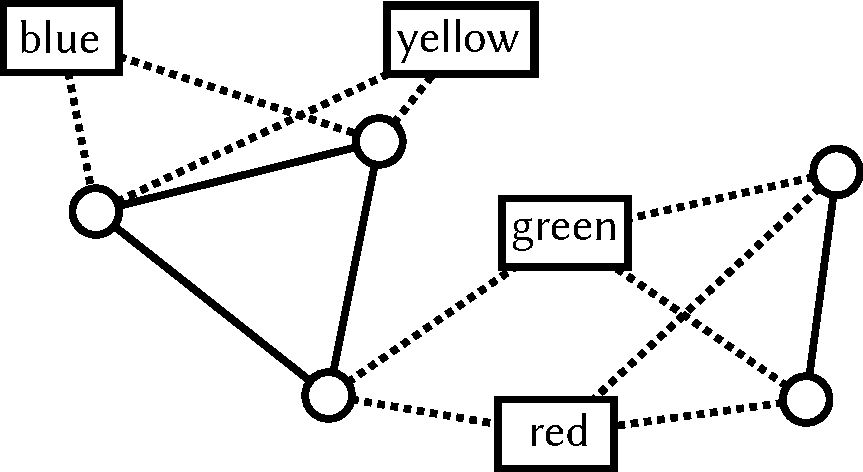
\includegraphics[width=\textwidth]{pix/SA2.pdf}
		%\caption{Simple graph}
		%\label{fig:gull}
	\end{subfigure}
	%\hfill
\caption[Transition to the augmented graph.]{Example of nodes with tags, and the corresponding augmented graph.}\label{fig:sa}
\end{figure}
%

The distance between two nodes is now determined by a random walk. A random walk model on a graph starts at a node $v_i$ and then follows $l$ edges at random; $l$ is called the length of the walk. A possibility distribution about how likely other nodes are reached emerges when this is done often enough. By assigning each edge $e_{i\,j}$ a possibility $w_{i\,j} = p_{i\,j}$ describing how likely this edge is used to transition to the next node, the possibility distribution can be calculated by summing up all probabilities of every path with length $l$.

\begin{align}
p(\tau) &= \prod_{e \in \tau} p(e)
\end{align}
%
Summing up all paths between two nodes $v_i$ and $v_j$ with length $l$:
\begin{align}
p(v_i, v_j)=\sum_{\substack{\tau: v_i \leadsto v_j\\lenght(\tau) = l}} p(\tau)
\end{align}
%
is the specific probability of reaching $v_j$ from $v_i$ through paths of length $l$.


%Example:
\begin{figure}%[h]
		\centering
		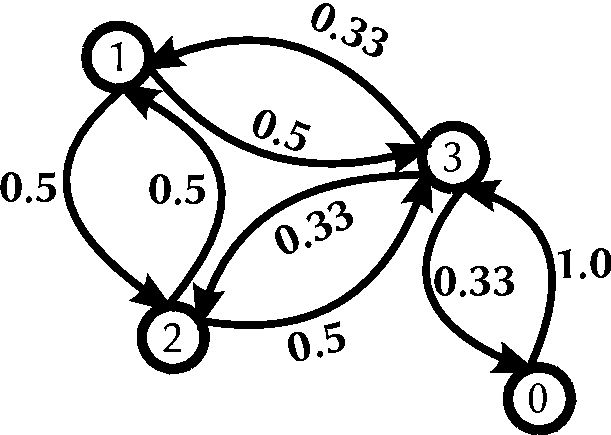
\includegraphics[width=0.5\textwidth]{pix/transition_ex.pdf}
		\caption[Graph with transition probabilities.]{Example graph with transition probabilities.}
		\label{fig:graph_for_examples}
\end{figure}

As an example this is shown in table~\ref{tbl:RW} for different path lengths based on the example graph in figure~\ref{fig:graph_for_examples}. The distribution diverges after a few iterations, regardless of where the walk was started. In this particular case, the probabilities diverges towards $[0.125, 0.250, 0.250, 0.375]$.

Having probabilities for choosing edges, independent of earlier transition choices makes this a \emph{markov chain}\cite{Aldous2002}. The adjacency matrix can also be called markov matrix, transition matrix or probability matrix $P$, because $w_{i\,j} = p_{i\,j}$. Markov chains as stochastic processes are well understood, thus every probability $p(v_j, v_i, l)$ of reaching $v_j$ from $v_i$ in a random walk with length $l$ can be calculated trough simple matrix multiplications of the transition matrix:

\begin{align}
p(v_j, v_i, l) &= P^l (v_j, v_i)
\end{align}

Table~\ref{tbl:RW2} shows an example of this using the transition matrix instead of finding and listing all possible paths. It can be seen that the distributions are very inconsistent in the first iterations, even on this small graph. The probability distribution which diverges over time is obviously no good indication of a distance between nodes.

Finally the distance between two nodes $f(v_i, v_j)$ based on a random walk model is the sum of each distribution for a finite number of iterations $l$ (which also means the sum of every possible path $\leq l$):

\begin{align}
f(v_i, v_j) &= \sum_{\substack{\tau: v_i \leadsto v_j\\lenght(\tau) \leq l}} p(\tau) \: c \: (1-c)^{lenght(\tau)}
\end{align}
%
or in matrix form
\begin{align}
R^l &= \sum^{l}_{y=1} c \: (1-c)^y \: P^y\\
		&= c \: (1-c)^l \: P^l + R^{l-1}
\end{align}
%
$c \in (0,1)$ is called restart probability and models the case that the random walker just stops. Because $w_{i\,j}$ is not necessary equal to $w_{j\,i}$, the resulting distance may differ $d(v_i, v_j) \overset{?}{=} d(v_j, v_i)$. To keep it simple, every distance is the average of $d(v_j, v_i)$ and $d(v_i, v_j)$ (respectively $R_d = \frac{R+R^T}{2}$). In table~\ref{tbl:RW3} the final distances for the example graph by using the random walk model can be found.

\section{Edge weights}
Assignment of the edge weights is based on the individual number of edges per attribute and node, and attribute weights for each attribute. There is a distinction between nodes and attributed nodes (edges) in calculating the edge weights. Therefore, the normal nodes are called structure nodes ($v_i, v_j$), and the nodes generated from the attributes are called augmented nodes ($v_k^a$). $v_k^a$ describes the node based on the $a^{th}$ value of attribute $k$. Similarly $v_k$ is the set of all nodes based on attribute $k$. There are edges $(v_i, v_k^a), (v_k^a, v_i)$ if and only if $v_i$ has the $a^{th}$ value of attribute $k$ set. Structure edges have an attribute weight of $\omega_0$, while the augmented edges of attributes $k_1, \dots, k_m$ have attribute weights $\omega_1, \dots, \omega_m$.

\subsubsection*{Example}
Node $v_{42}$ has the attribute $text = [red, green]$. This means there are augmented nodes $v_{text}^{red}$ and $v_{text}^{green}$ with edges $(v_{42}, v_{text}^{red}), (v_{42}, v_{text}^{red}) \in E$. There are of course also edges from the augmented nodes to the structure node, but with different weights. See also for example figure~\ref{fig:sa}.
%The number of text edges for $v_{42}$ is written as $|N(v_{text})(v_{42})|$ and would be $2$.

\vspace{1em}
\noindent
The following transition probabilities are the edge weights between nodes as defined by \textcite{Zhou2009}. $|N(v)|$ is the number of outgoing edges of $v$.
%
\begin{align}
\intertext{structure edge $(v_i, v_j)$}
w_{v_i \, v_j} &=
\begin{cases} 
	\frac{\omega_0}{|N(v_i)| \, \cdot \, \omega_0 + \omega_1 + \dots + \omega_m} &\text{if } (v_i,v_j) \in E\\
	0 &otherwise
\end{cases}
\intertext{attribute edge $(v_i, v_k^a)$}
w_{v_i \, v_k^a} &=
\begin{cases} 
	\frac{\omega_k}{|N(v_i)| \, \cdot \, \omega_0 + \omega_1 + \dots + \omega_m} &\text{if } (v_i,v_k^a) \in E\\
	0 &otherwise
\end{cases}
\intertext{attribute edge $(v_k^a, v_{j})$}
w_{v_k^a \, v_{j}} &=
\begin{cases} 
	\frac{1}{|N(v_k^a)|} &\text{if } (v_k^a, v_{j}) \in E\\
	0 &otherwise
\end{cases}
\end{align}
%
There are no edges between attribute nodes.

The edge weights $w_{i\,j}$, thus $P_A$, should represent a probability distribution with the requirements $0 \leq w_{i\,j} \leq 1$ and $\sum_{j} w_{i\,j} = 1$. All edges from attribute nodes obviously fulfil this requirement. But edges from structure nodes have various summed probabilities. This will be exemplary shown after the following proposed edge weights. $N_k(v_i)$ is the number of edges to any attribute node $v_k^a$; similarly $N_0(v_i)$ for edges to structure nodes. 
%
\begin{align}
\intertext{structure edge $(v_i, v_j)$}
w_{v_i \, v_j} &=
\begin{cases} 
	\frac{\omega_0}{\sum_m \omega_m |N_m(v_i)|} &\text{if } (v_i,v_j) \in E\\
	0 &otherwise
\end{cases}
\intertext{attribute edge $(v_i, v_k^a)$}
w_{v_i \, v_k^a} &=
\begin{cases} 
	\frac{\omega_k}{\sum_m \omega_m |N_m(v_i)|} &\text{if } (v_i,v_k^a) \in E\\
	0 &otherwise
\end{cases}
\end{align}
%
Attribute weights now proportionally control the different edge weights.

\subsubsection*{Example}
This example demonstrates the difference between the old edge weights as described in \cite{Zhou2009} and the new proposed edge weights. The basis is a node with 3 structure edges and 6 attribute edges of attribute 1. Attribute weights are $\omega_0 = 0.7, \omega_1 = 0.3$. This results in the following weights per edge respectively the sum of the probabilities:


\begin{center}
\footnotesize
\begin{tabular}{rrrr}
\toprule
 & $w_{structure}$ & $w_{attribute}$ & $\sum_{j} w_{i\,j}$\\
\midrule
old & $0.106$ & $0.045$ & $0.59$\\
new & $0.179$ & $0.077$ & $1.00$\\
\bottomrule
\end{tabular}
\end{center}
%
Attribute edge weights can be any positive number.

\section{Super nodes}
The proposed calculation scheme based on matrix multiplications is easy to adopt, because there are many fast and relatively easy to use libraries dealing with (sparse) matrix multiplication.

Dealing with datasets containing hundreds of thousands, or millions of documents require huge amounts of memory when using matrix multiplications. 
For example a full matrix of 25,000 points with single-precision floating point numbers (32~Bit) , needs approximately 4.6~GB of space. This number grows quadratic with the count of documents. Even with sparse matrices, which store only values other than $0$, the matrices grow very big after a few iterations of multiplications. Too big for the test system in use with 4~GB RAM.

The datasets used have an interesting characteristic: many points with the same attributes are at the same position (or at least less than a few meters apart). It is safe to assume that they end up in the same cluster. All this occurrences of structure nodes with the exactly same attributes within very close proximity are in each case combined to super nodes.

The idea behind super nodes is to reduce the amount of nodes and edges in the graph, thus reducing the space needed, without changing the local characteristics of the edges and their weights to much. Incoming\,/\,outgoing edges involving the same node are being merged. Every incoming edge now represents $k$ normal edges, and has $k$-times the priority of a normal edge. $k$ is based on the number of nodes $N_w$ consolidated by the super node based on the following equation:

\begin{align}
k =  \frac{\sqrt{9 \cdot N_w}}{2}
\end{align}
%
Without this adjustment the super nodes gained too much incoming probability, leading to low distances to super nodes, but to high to other nodes. Edges to and from augmented nodes are handled the same way. Figure~\ref{fig:w_nodes} shows this concept.

Using super nodes helped to reduce the needed amount of memory drastically, so that even one million points can be computed with the test system. Previously this had theoretically required over 7~TB of RAM.

\begin{figure}[h]
\centering
	\begin{subfigure}[b]{0.4\textwidth}
		\centering
		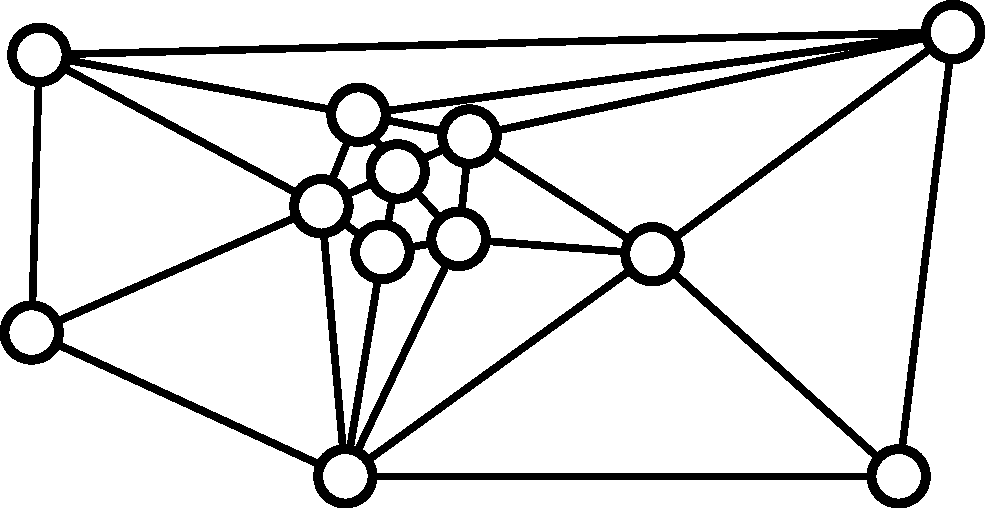
\includegraphics[width=\textwidth]{pix/w_nodes1.pdf}
		%\caption{Simple graph}
		%\label{fig:gull}
	\end{subfigure}
	\hfill
	\begin{subfigure}[b]{0.4\textwidth}
		\centering
		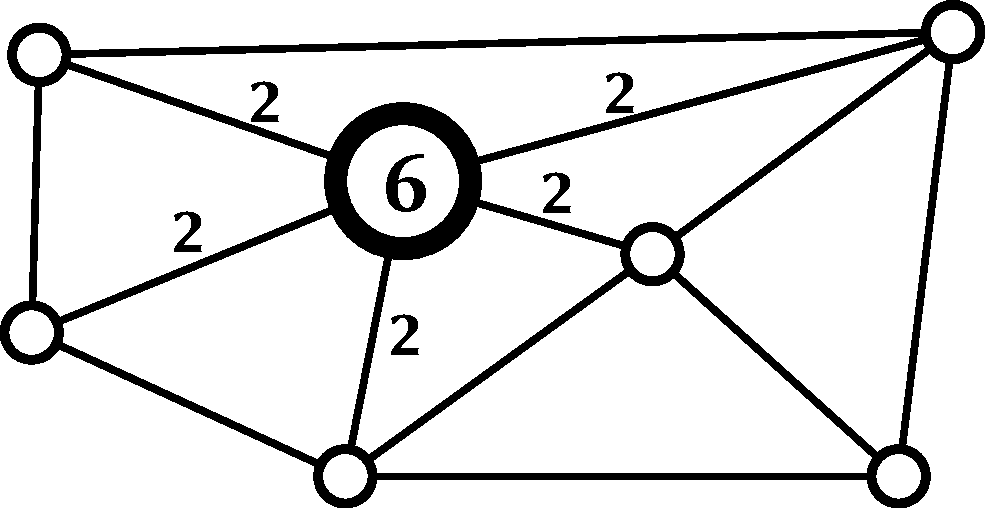
\includegraphics[width=\textwidth]{pix/w_nodes2.pdf}
		%\caption{Simple graph}
		%\label{fig:gull}
	\end{subfigure}
	%\hfill
\caption[Transition from normal nodes to a super node.]{Example of a transition from normal nodes to super nodes. All edges count as 1, except for the ones from and to the newly created super node.}\label{fig:w_nodes}
\end{figure}

\section{Generating the graphs}\label{sec:graph_generation}
The described graph algorithm operates on a structure graph based on the location data and different augmented graphs for every other used attribute (text data in this case). Creating the augmented graphs is easy: 
\begin{enumerate}
\item Create an augmented node for every individual value of every attribute
\item Create edges between structure nodes and augmented nodes
\end{enumerate}
%
That is all to represent the relationship between structure node and augmented node. The relationship between structure nodes should be based upon the closeness of each other and the relative density of the points. This means, there should be no edge between nodes to far away, and there should be a rather high connectivity in areas with many points.

The following two approaches come to mind, where an edge is created to either 
\begin{enumerate}
\item all the $n$-nearest nodes, or 
\item all nodes in an $eps$-neighbourhood.
\end{enumerate}
%
Both reflect the closeness and density aspects, but unfortunately suffer for these exact same reasons. They usually connect highly in dense areas, but very little elsewhere. Connectivity sometimes reached a point where every node in an area was connected to every other node. Which did not work well for the algorithm, was calculation intensive, and reduced the meaning (closeness) of an edge. 

Beside this general problem, approach 1 sometimes forms \enquote{bubbles}: sets of highly interconnected nodes without edges to surrounding nodes, in high density areas. Raising $n$ would prevent this, at the cost of even greater interconnected areas. And approach 2 was very sensitive in choosing $eps$. Nodes inside a neighbourhood were usually very highly interconnected; nodes outside very usually not connected at all.\footnotetext[3]{\url{https://en.wikipedia.org/wiki/File:Delaunay_circumcircles.png}}

\begin{wrapfigure}{r}{0.42\textwidth}
	\centering
	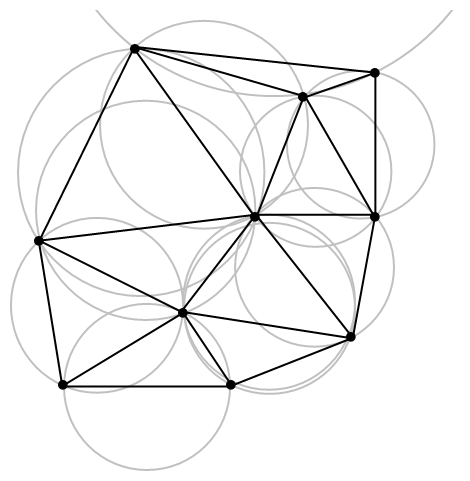
\includegraphics[width=0.38\textwidth]{pix/Delaunay_circumcircles.png}
	\caption[Delaunay triangulation example]{Delaunay triangulation example{\protect\footnotemark}}
	\label{fig:delaunay_example}
\end{wrapfigure}
%
Because of those problems, the final method of creating the structure graph is a \emph{Delaunay triangulation}. A triangulation is a set of non-intersecting edges, whose only shapes are triangles. A Delaunay triangulation is a special triangulation, such that no node is inside the circumcircle of any triangle. A circumcircle is the circle whose center is equidistant to all three points of the triangle. Figure~\ref{fig:delaunay_example} shows an example together with the circumcirles of the triangles. Because of this requirement the minimum angle of all the angles of the triangles is maximised. This results in well distributed looking edges, whose nodes are close to each other, without too much interconnectivity in highly populated areas. 

Areas with low point density will also be well connected. This is a problem, because those points can be rather far away from each other. Deleting edges above a certain threshold lowers this and results are much better, but the bottom line is:

The case of extreme connectivity versus no connectivity, in both approaches \enquote{$n$-nearest nodes} and \enquote{$eps$-neighbourhood}, is now traded to good connectivity versus mild connectivity. Examples of the triangulations, together with colour-coded edge lengths can be seen in the description of the datasets in section~\ref{sec:datasets}.%\todo{more DT}


\chapter{Evaluation and comparison}
\emph{%
This chapter begins with the introduction of the used evaluation measurements including a comparison of their strengths and weaknesses based on artificial datasets. Then a recap of all used parameters for DBSCAN and the distance metrics are given. This is followed by the description of the datasets used for the overview of the good and the bad of the two distance metrics, which concludes this chapter.
}\label{chap:eval}

\section{Evaluation measures}\label{sec:cqm}
Cross validation\cite{Park2009} is a common evaluation technique  of probabilistic models as seen in some related works\cite{Hong2012, Yin2011}. There are many different ways to cross validate, but the general idea stays the same: generate the model based on based on a part of the dataset (model set), and evaluate with another (test set), for example with perplexity, or by measuring the average error between predicted location and real location. This is usually done to ensure that the generated model is able to classify previously unknown documents respectively that the model is not to specific to the documents used for generation.

This form of evaluation can hardly be applied to clustering tasks, because their is no standard way to classify unknown, unused objects to an existing clustering; other than to cluster the data again. Therefore there are other evaluation measures, which could also be used with probability models. Clustering evaluation measures try to measure the goodness of a clustering. Because the \enquote{goodness} is usually domain and task dependent, there are many different cluster quality measures (CQM).

%external
A rough classification of the different quality evaluation measures would group them into either \emph{external} or \emph{internal} quality measures\cite{Rendon2011}. External indices use domain or a priori knowledge. The two popular external measures \emph{precision} and \emph{recall} for example are using existing and correct classification information of datasets (also called gold standards) and are calculated by using the number of items correctly (or falsely) labelled. 
%f-scan

%internal
Internal evaluation measures only use the information provided by the dataset itself. This boils mostly down to using either the \emph{compactness} or the \emph{separability} of the resulting clustering, or both.
%
Compactness measures the closeness of elements in a cluster, while separability indicates how distinct two clusters are by computing the distance between two different clusters.

Datasets containing a priori knowledge usable for external evaluation measures are generally either artificial or hand annotated; meaning that most real problems and natural datasets contain no external knowledge for external evaluation measures.  Therefore the following indices used in this thesis are all internal evaluation measures.
%\newpage

\subsection{Dunn index}
The Dunn index\cite{Dunn1973} $D$ defines the ratio between the minimal inter cluster distance to the maximal intra cluster distance.

\begin{align}
D = \frac{d_{min}}{d_{max}},
\end{align}
%
where $d_{min}$ denotes the smallest distance between two objects from different clusters, and $d_{max}$ the largest distance of two objects from the same cluster.

\vspace{.5em}
\noindent
The Dunn index is limited to the interval $[0, \infty]$ and should be maximized.


\subsection{Davies-Bouldin index}
The Davies-Bouldin index\cite{Davies1979} $DB$ is defined as:

\begin{align}
DB = \frac{1}{n} \sum^n_{i=1, i \neq j} max(\frac{\rho_i + \rho_j}{d(center_i, center_j)})
\end{align}
%
where $n$ is the number of clusters, $\rho_i$ is the average distance of all documents in cluster $c_i$ to their cluster center $center_i$ and $d(center_i, center_j)$ is the distance of the two cluster centers $center_i$ and $center_j$. Small values of $DB$ correspond to clusters that are compact, and whose cluster centers are far away from each other.

\vspace{.5em}
\noindent
The Davies-Bouldin index is limited to the interval $[0, \infty]$ and should be minimized.

\subsection{C-index}
The C-index\cite{Hubert1976} $C$ is defined as:
\begin{align}
C = \frac{S - S_{min}}{S_{max} - S_{min}},
\end{align}
%
where $S$ is the sum of distances over all pairs of objects from the same cluster, $n$ is the number of those pairs and $S_{min}$ is the sum of the $n$ smallest distances if all pairs of objects are considered. Likewise $S_{max}$ is the sum of the $n$ largest distances out of all pairs.

\vspace{.5em}
\noindent
The C-index is limited to the interval $[0, 1]$ and should be minimized.


%Boros-Clustering-2011-May-24
\subsection{Silhouette width}
The silhouette width\cite{Rousseeuw1987} $SW_i$ indicates how well element $i$ was clustered.

\begin{align}
SW_i = \frac{b_i-a_i}{max(a_i, b_i)},
\end{align}
where $a_i$ is the average distance from point $p_i$ to all other points in his cluster, and $b_i$ is the minimum average distance from point $p_i$ to all points in the another clusters. The average silhouette width $ASW$ then measures the global goodness of a clustering.

\begin{align}
ASW = \frac{\sum_i SW_i}{n}
\end{align}

\vspace{.5em}
\noindent
The average silhouette width is limited to the interval $[-1, 1]$ and should be maximized.

\subsection{Quality check}\label{sec:qcheck}
Unfortunately these quality measures have their strengths and weaknesses. Those will be explored based on artificial datasets. These CQMs are useful at comparing different clusterings, but can they also be used to indicate a global goodness?

Figure~\ref{fig:clusterexamples} shows four synthetic point arrangements coloured after their cluster categorisation, while table~\ref{tbl:syn_compare} lists the respective measurement scores.
\begin{description}
\item[blobs] shows three clearly distinguishable point clusters
\item[random] shows points randomly distributed in space; the clustering is also random in this case
\item[moons] shows two half-moon shaped point arrangements
\item[circles] shows two rings, a small one inside a bigger one
\end{description}

\begin{figure}%[hbt]
\centering	
	\begin{subfigure}[b]{0.22\textwidth}
		\centering
		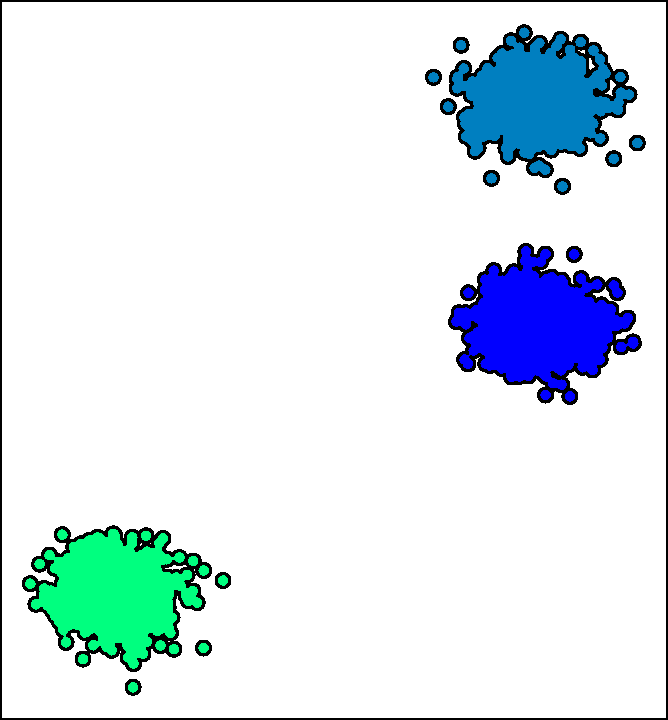
\includegraphics[height=\textwidth]{pix/blobs_color_3600.pdf}
		\caption{blobs}
	\end{subfigure}
	\hspace*{0.01\textwidth}	
	\begin{subfigure}[b]{0.22\textwidth}
		\centering
		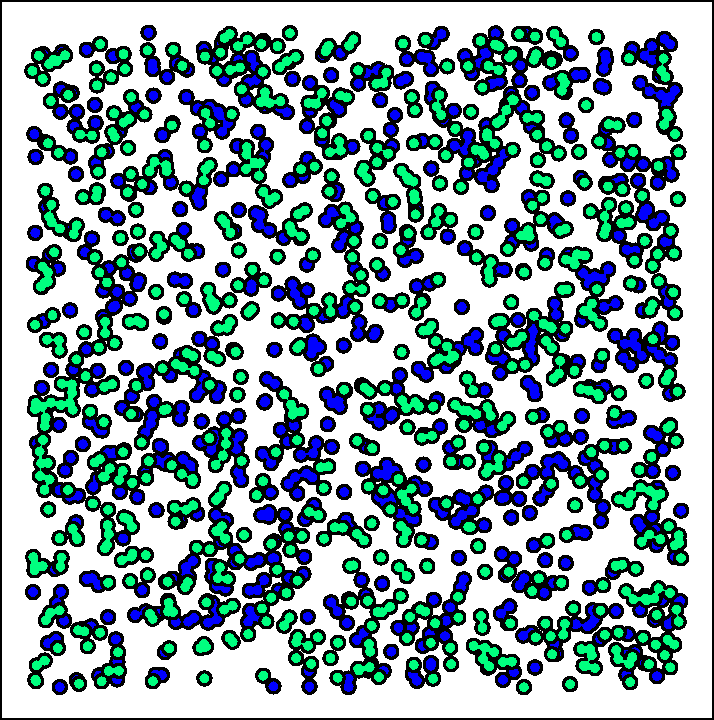
\includegraphics[height=\textwidth]{pix/random_color_3600.pdf}
		\caption{random}
	\end{subfigure}
	\hspace*{0.015\textwidth}	
	\begin{subfigure}[b]{0.22\textwidth}
		\centering
		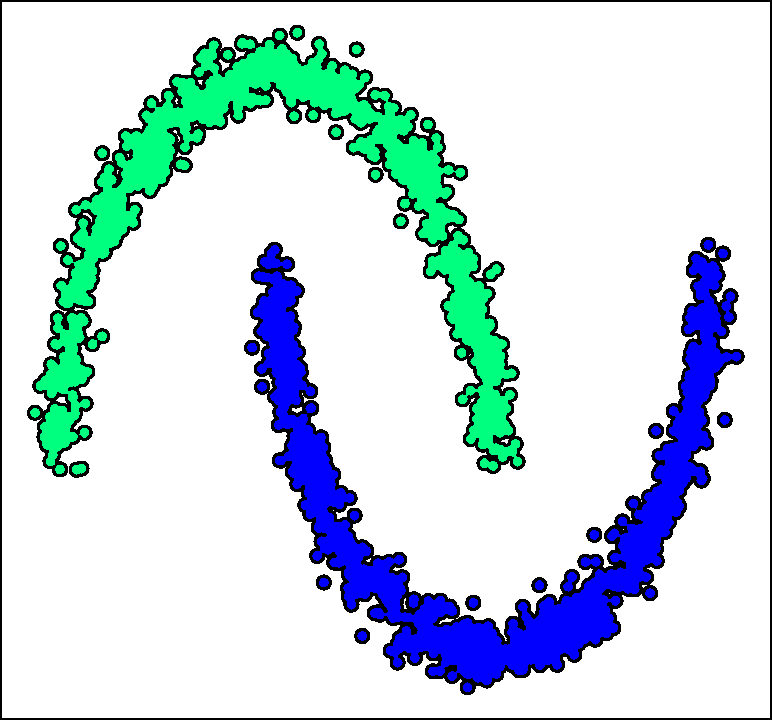
\includegraphics[height=\textwidth]{pix/noisy_moons_color_3600.pdf}
		\caption{moons}
	\end{subfigure}
	\hspace*{0.035\textwidth}	
	\begin{subfigure}[b]{0.22\textwidth}
		\centering
		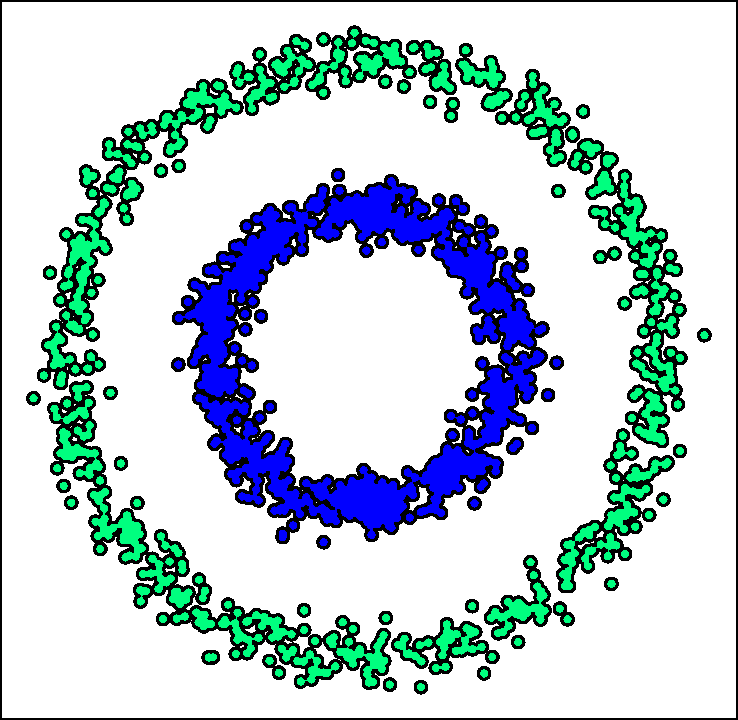
\includegraphics[height=\textwidth]{pix/noisy_circles_color_3600.pdf}
		\caption{circles}
	\end{subfigure}    
\caption{Synthetic clustering examples}\label{fig:clusterexamples}
\end{figure}
%\begin{figure}[Hht]
%\centering
%	\begin{subfigure}[b]{0.3\textwidth}
%		\centering
%		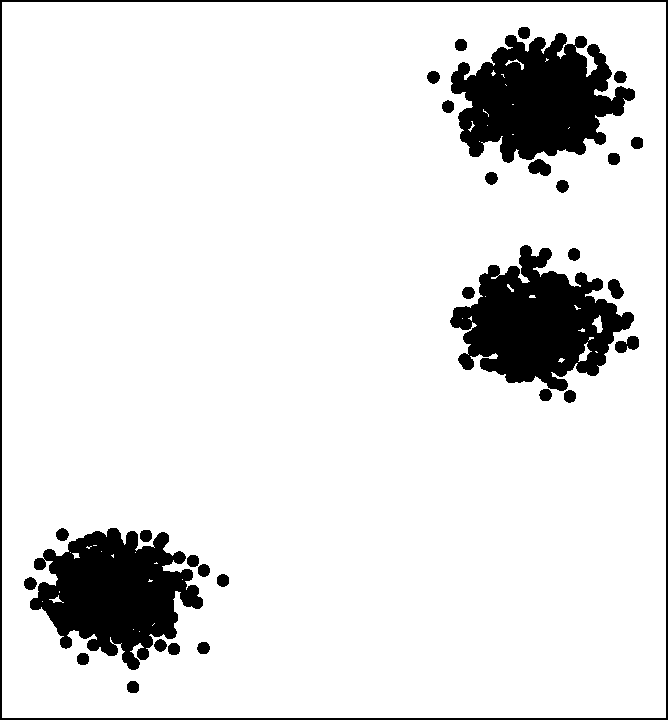
\includegraphics[width=\textwidth]{pix/blobs_scatter.pdf}
%		%\caption{Blobs}
%		%\label{fig:gull}
%	\end{subfigure}
%	\,
%	\begin{subfigure}[b]{0.3\textwidth}
%		\centering
%		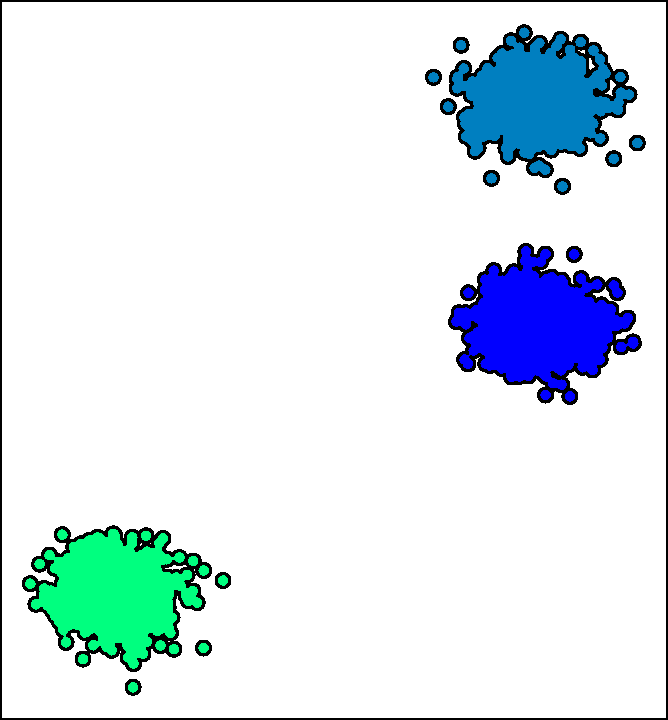
\includegraphics[width=\textwidth]{pix/blobs_color_3600.pdf}
%		%\caption{Random}
%		%\label{fig:gull}
%	\end{subfigure}
%	
%	\hfill
%	
%	\begin{subfigure}[b]{0.3\textwidth}
%		\centering
%		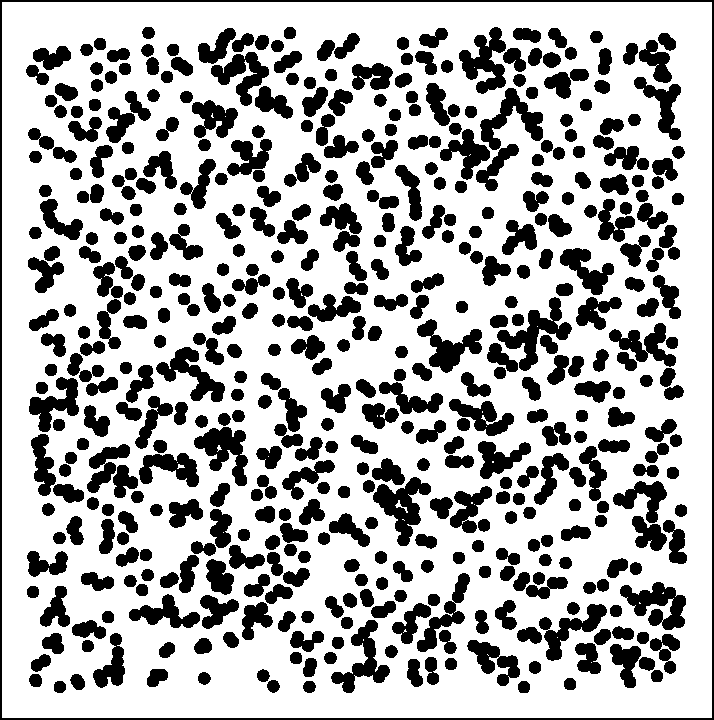
\includegraphics[width=\textwidth]{pix/random_scatter.pdf}
%		%\caption{Random}
%		%\label{fig:gull}
%	\end{subfigure}
%	\,
%	\begin{subfigure}[b]{0.3\textwidth}
%		\centering
%		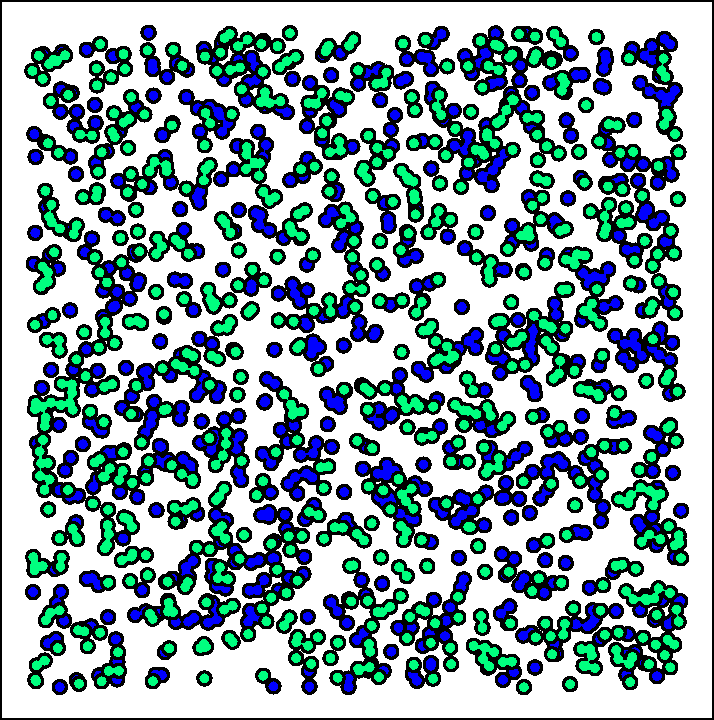
\includegraphics[width=\textwidth]{pix/random_color_3600.pdf}
%		%\caption{A gull}
%		%\label{fig:gull}
%	\end{subfigure}
%
%	\hfill
%
%	\begin{subfigure}[b]{0.3\textwidth}
%		\centering
%		
\includegraphics[width=\textwidth]{pix/noisy_moons_scatter.pdf}
%		%\caption{Half-moons}
%		%\label{fig:gull}
%	\end{subfigure}
%	\,
%	\begin{subfigure}[b]{0.3\textwidth}
%		\centering
%		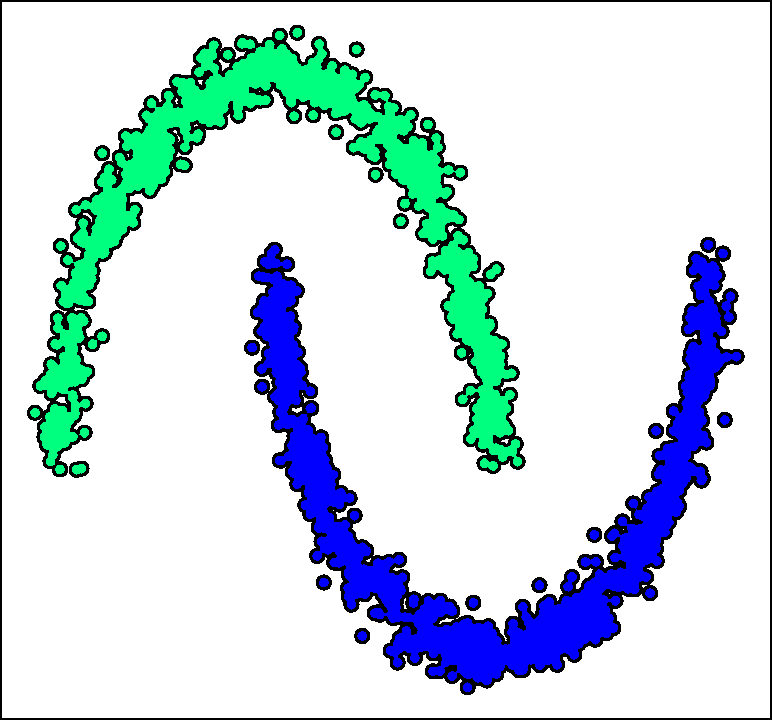
\includegraphics[width=\textwidth]{pix/noisy_moons_color_3600.pdf}
%		%\caption{A gull}
%		%\label{fig:gull}
%	\end{subfigure}
%
%	\hfill
%
%	\begin{subfigure}[b]{0.3\textwidth}
%		\centering
%		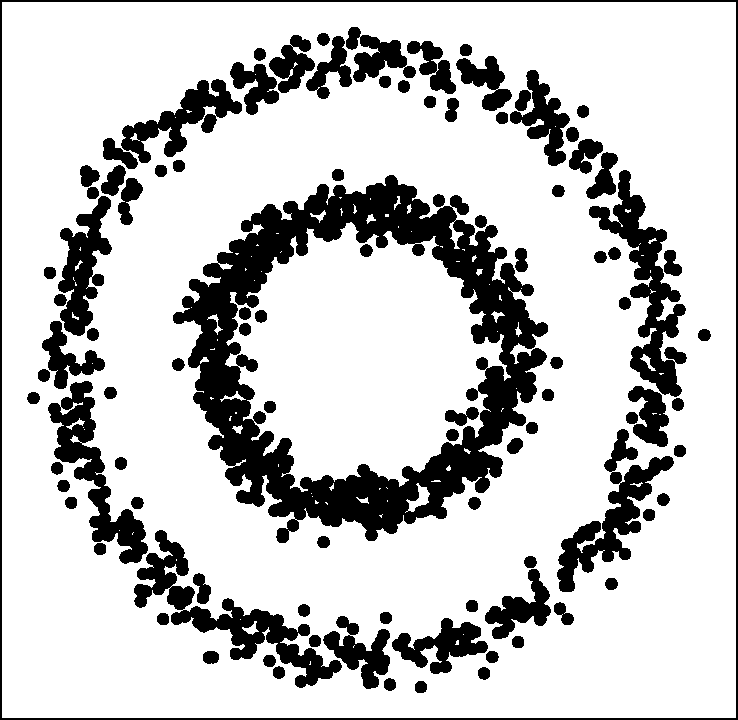
\includegraphics[width=\textwidth]{pix/noisy_circles_scatter.pdf}
%		%\caption{Circles}
%		%\label{fig:gull}
%	\end{subfigure}
%	\,
%	\begin{subfigure}[b]{0.3\textwidth}
%		\centering
%		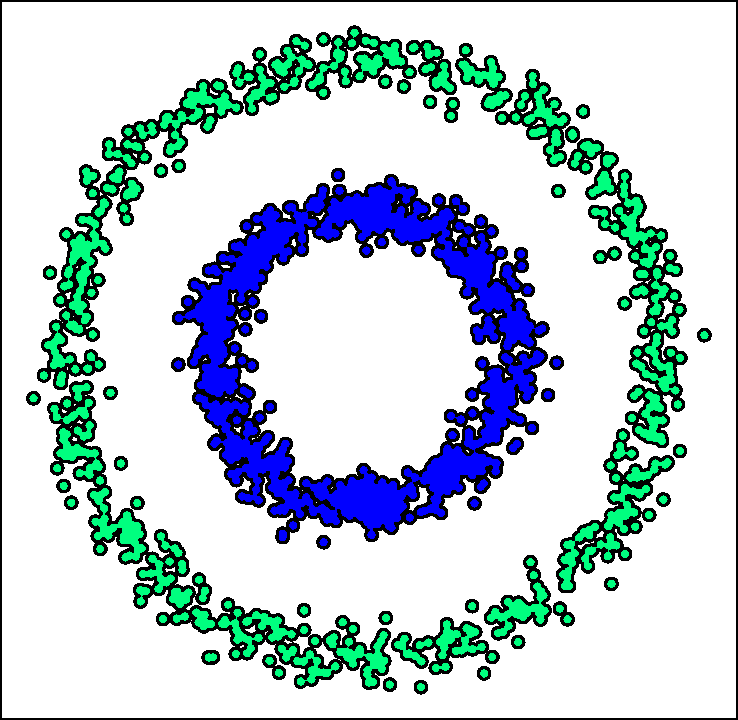
\includegraphics[width=\textwidth]{pix/noisy_circles_color_3600.pdf}
%		%\caption{A gull}
%		%\label{fig:gull}
%	\end{subfigure}        
%\caption{Synthetic clustering examples}\label{fig:clusterexamples}
%\end{figure}

\begin{table}%[bth]
\caption{Comparison of the evaluated synthetic test cases}\label{tbl:syn_compare}
\centering
\sisetup{table-format = 1.0(1)e2}
\begin{tabular}{cSSSS}
\toprule
Dataset & {DB} &{C}&{SW}&{D}\\
			& {\scriptsize $0<min<\infty$} &{\scriptsize $0<min<1$}&{\scriptsize $-1<max<1$}&{\scriptsize $0<max<\infty$}\\
\midrule
blobs	& 1.35e-02 & 3.18e-09 & 9.87e-01& 3.13e+00\\
circles	& 1.36e+00& 5.01e-01 & 1.11e-01 & 1.43e-02\\
moons	& 3.31e-01 & 1.50e-01 & 5.25e-01 & 5.01e-02\\
random& 5.29e+01 & 5.00e-01 & 1.91e-03 & 9.67e-07\\
\bottomrule
\end{tabular}
\end{table}
%
\newpage
It is obvious that those clusters are optimal. Sadly every cluster measurement fail in one way or another. Except 
\begin{description}
\item[DB,] which shows a bad result for $random$, and good ones for the others. $circles$ is here a little worse than $blobs$ and $moons$, because its two cluster centers are very close to each other.

\item[C] indicates a good results for $blobs$ and $moons$, but regards $circles$ and $random$ equally mediocre, but nor really bad either. It seems they both share the same ratios of minimum to maximum distances and their respective sums.

\item[SW] performs well for $blobs$ and $moons$. But less well for $circles$---the average distances to the two clusters seem not too be that far apart. The $random$ clustering scores as expected; its average distances should be the same for the two randomized clusters.

\item[D] scores $blobs$ really high, but not the rest. Big or widespread clusters have higher maximum distances. When those clusters are fairly near together, their score drops significantly.
\end{description}
%
After this short test comparison, it should be clear to not trust those scores blindly. A few more aspects of how a good clustering should look are now presented. These are very subjective aspects, and will differ from case to case. But they help to address different points of views and to discuss those, if needed.
%
\begin{description}
\item[Noise] The amount of documents regarded as $noise$ should not be high. There could always be documents which do not fit to the available clusters, but $noise$ should be minimized, either through better distance functions or a better dataset. $noise$-threshold in this thesis is set to the arbitrary amount of maximal a quarter of the dataset size.
\item[Number of clusters] Some algorithms, like k-means, need this as a parameter. A common approach is to use a CQM and take the amount of clusters which maximises the score. This can work, if the CQM is carefully chosen. Arbitrary baseline is, that there should be 2 order of magnitudes between the size of the dataset and the number of clusters.
\item[Items per cluster] The distribution of items per cluster is also to take into account. The best case is an even distribution (every cluster has the same size). But this is unfortunately never the case. A power-law distribution is more common, where the most documents are clustered in a very few clusters.
\end{description}
%
The search for good clusters is after all very subjective and depended on domain knowledge. But rules for filtering the worst results on the considerations above are easy to write.

\section{Parameter choice}
The choice of the parameters used for creating the clusterings that are going to be compared is very crucial. To present a clear picture about the possibilities of the evaluated algorithms, or distance metrics, the parameters delivering the best results should be always used. But finding these parameters in a reasonable time is not always possible. 

Because of that, the time and effort of finding good setting should either be quantitatively reflected in the final verdict, or be equally distributed between the candidates. The later is usually done, by using domain knowledge and common sense for the parameter choice.

Presented now is a recap of all the available parameters which have influence on the cluster results and explanations for the values used.

DBSCAN has the two parameters $eps$ and $minPts$, which describe how much points ($minPts$) have to be at least in an $eps$-neighbourhood of a point for it to be considered dense and part of a cluster. The usual approach is to lock $minPts$ and experiment with $eps$.
%
\begin{align*}
minPts &= 4 & eps_{DBSCAN} &= \dots\\
\intertext{The combined distance has weight and threshold parameters for normalising the distances. The idea behind the normalization is, to get exactly $1.0$ if both distances are equal to their thresholds. Therefore $eps_{DBSCAN}$ is set to $1.0$. Weights and thresholds are both multiplied with each other, so we lock the weights to $0.5$ and experiment with the thresholds.}
eps_{DBSCAN} &= 1.0\\
w_{text} &= 0.5	&	w_{location} &= 0.5\\
eps_{text} &= [0.1, 0.5, 0.9] & eps_{location} &= \dots\\
\intertext{The random walk distance has parameter controlling the generation and weights of the graph. Here is no easy normalisation scheme, thus $eps_{DBSCAN}$ is used as intended for experimentation. The weights of the attributes are relative to each other, therefore $w_{location}=1.0$, while $w_{text}$ is set to different values. Edges which are too long can be removed from the graph based $km$. This value is based on the visual impression regarding the overall distribution of short and long edges; visualisations can be seen in figures~\ref{fig:A}, \ref{fig:B} and \ref{fig:C}. Finally there is $c=0.1$ and $l=20$. $c$ is the restart probability and $l$ the length of the random walk. Both are set as described in \cite{Zhou2009}.}
eps_{DBSCAN} &= \dots & km &= \text{based on visual impression}\\
c &= 0.1 & l &= 20\\
w_{text} &= [0.1, 1.0, 2.0] & w_{location} &= 1.0
\end{align*}
%
The search ranges (noted above as $\dots$) are manually explored with the settings above, based on the considerations from the previous section~\ref{sec:qcheck}. The best looking findings are then quantitatively measured with the described CQMs.

\section{Datasets}\label{sec:datasets}
For the comparison between the two approaches three datasets have been used. Table~\ref{tbl:datasets} shows the details. It can be seen that dataset A from Twitter has much more different words and points than B and C from Flickr, especially when considering the document size. This could result from the different usages of the services. Twitter user are much more mobile, and usually do not sent many tweets from the same location, while Flickr photos, when taken from the same spot, or geotagged afterwards, have much more locations in common. This results in a general different distribution of points in space and the generated graphs are much more sparse for B and C, as seen in figures~\ref{fig:A}, \ref{fig:B} and \ref{fig:C}. Dataset C was also used by \textcite{Sengstock2012a}.

The used words are also very different. While Flickr tags are more descriptive, Twitter tweets have much more abbreviated and strange words, due to the limitation on 140 characters per tweet. The usage again leads to very different characteristics as seen in table~\ref{tbl:top_words}. Datasets B and C have easy to recognise words, while A contains even numbers in its top ten of words. Word distributions are also very different. Having a few words with high count in contrast to the majority with low count is usual. This can be seen in B and C, where the tenth has approximately half the count of the first, but the distribution of A is very distorted, with the first having eight times the count of the tenth word. 

\begin{table}
\caption{Details of the datasets}\label{tbl:datasets}
\centering
\begin{tabular}{crrrcc}
\toprule
Dataset	& \# documents & \# unique points & \# words&source&general location\\
\midrule
A	& \num{57554}	&	\num{25665} & \num{30001}	&Twitter&Germany\\%Dataset Germany small
B	& \num{1254298}	&	\num{8831} & \num{3229} &Flickr&Germany\\%Dataset Germany
C	& \num{1086678}	&	\num{12992} & \num{4373} &Flickr&United States\\%Dataset USA small 1M
\bottomrule
\end{tabular}
\end{table}



%\afterpage{
\begin{figure}[p]
	\begin{subfigure}[b]{0.49\textwidth}
	\centering
	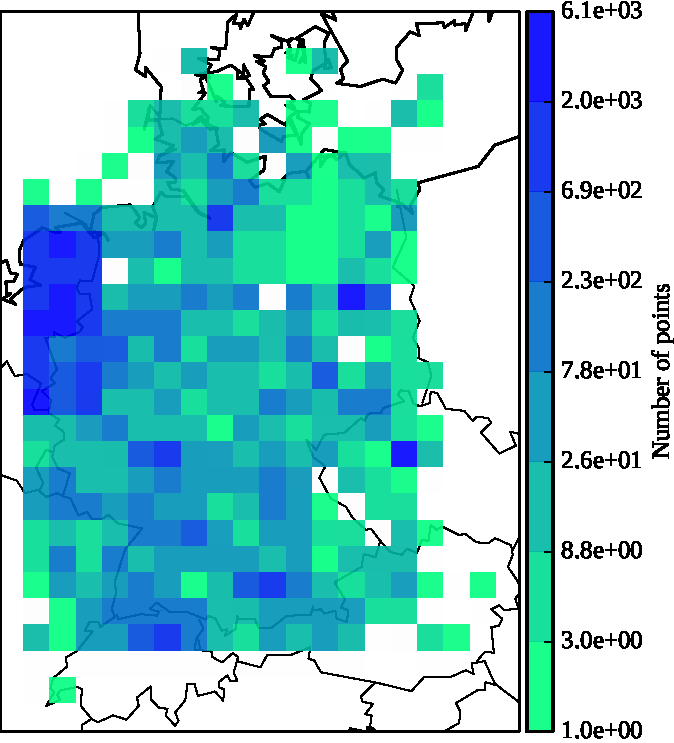
\includegraphics[width=.99\textwidth]{pix/freq_ger_small.pdf}
		\caption{Frequency plot}
		%\label{fig:gull}
	\end{subfigure}
	%
	\begin{subfigure}[b]{0.482\textwidth}
	\centering
	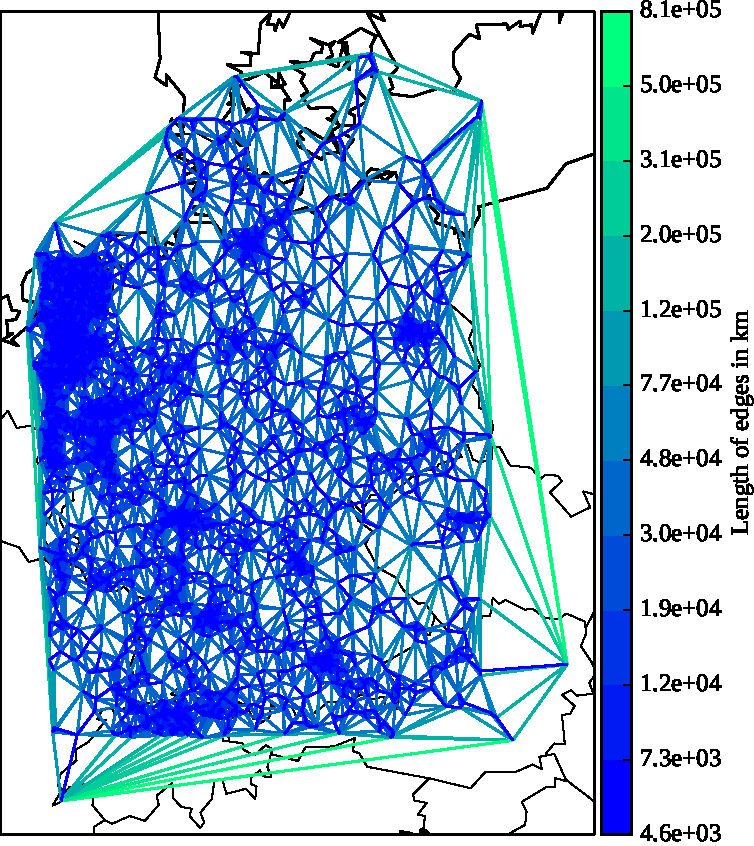
\includegraphics[width=.99\textwidth]{pix/tri_ger_small.pdf}
		\caption{Edge plot}
		%\label{fig:gull}
	\end{subfigure}
	\caption[Dataset A frequency and edge plots]{Dataset A pictures}
	\label{fig:A}
\end{figure}
%
\begin{figure}[p]
	\begin{subfigure}[b]{.49\textwidth}
	\centering
	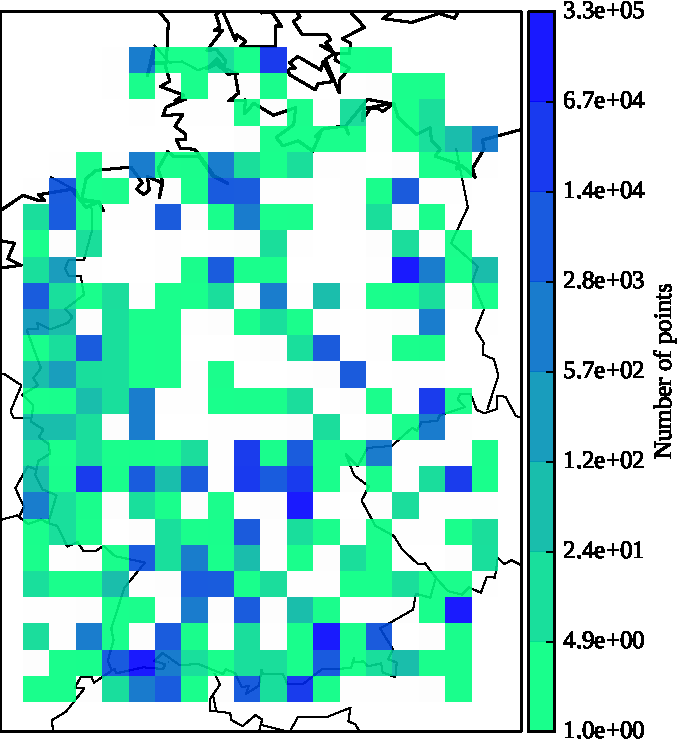
\includegraphics[width=.99\textwidth]{pix/freq_ger.pdf}
		\caption{Frequency plot}
		%\label{fig:gull}
	\end{subfigure}
	%
	\begin{subfigure}[b]{.482\textwidth}
	\centering
	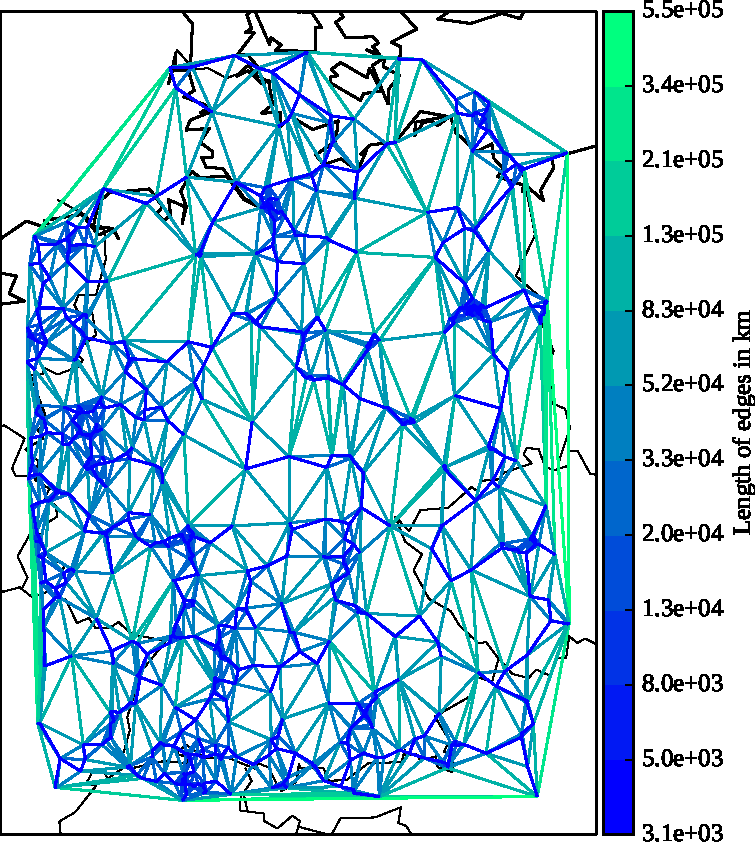
\includegraphics[width=.99\textwidth]{pix/tri_ger.pdf}
		\caption{Edge plot}
		%\label{fig:gull}
	\end{subfigure}
	\caption[Dataset B frequency and edge plots]{Dataset B pictures}
	\label{fig:B}
\end{figure}
%
%\clearpage
%}

%\afterpage{
\begin{figure}[p]
	\begin{subfigure}[b]{\textwidth}
	\centering
	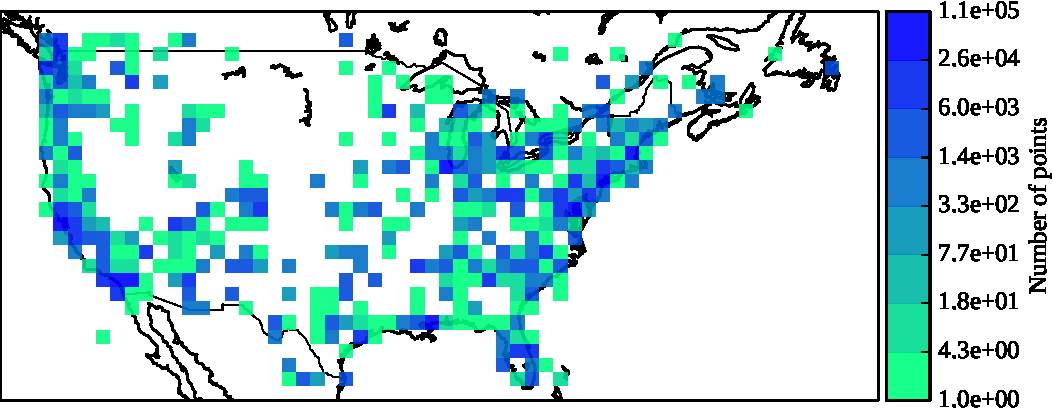
\includegraphics[width=1.\textwidth]{pix/freq_usa_small.pdf}
		\caption{Frequency plot}
		%\label{fig:gull}
	\end{subfigure}
	%
	\begin{subfigure}[b]{\textwidth}
	\centering
	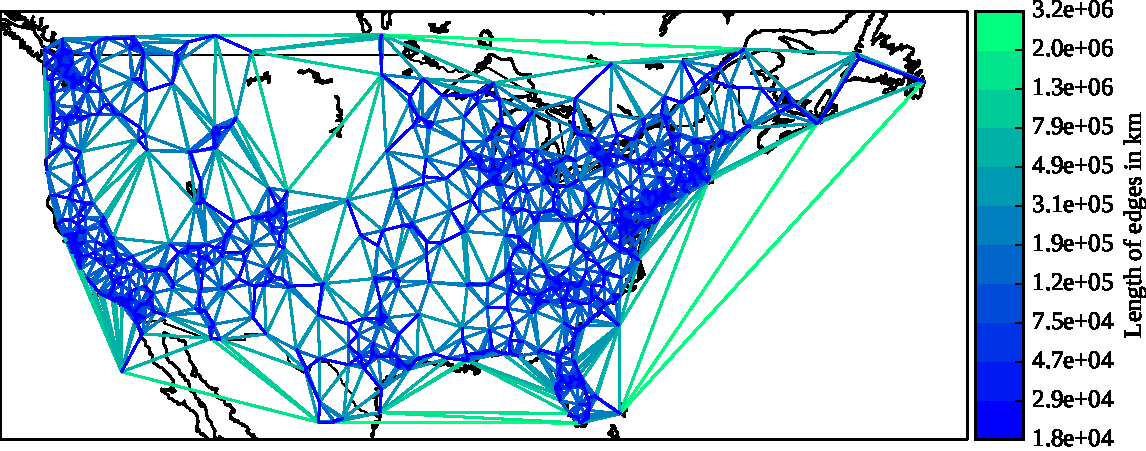
\includegraphics[width=1.\textwidth]{pix/tri_usa_small.pdf}
		\caption{Edge plot}
		%\label{fig:gull}
	\end{subfigure}
	\caption[Dataset C frequency and edge plots]{Dataset C pictures}
	\label{fig:C}
\end{figure}
%\enlargethispage{5\baselineskip}

%\begin{table}[htb]
%\caption{Ten most words in the datasets}
%\footnotesize
%\label{tbl:top_words}
%\begin{subtable}{.33\linewidth}
%\centering
%\begin{tabular}{cr}
%\toprule
%\multicolumn{2}{c}{dataset A}\\
%\midrule
%nowplaying & \num{4494}\\
%acakfilm & \num{4086}\\
%ger & \num{1666}\\
%pp11 & \num{1464}\\
%176 & \num{1242}\\
%brandenburg & \num{1107}\\
%twexit & \num{986}\\
%fb & \num{960}\\
%9748 & \num{728}\\
%bbradio & \num{656}\\
%\bottomrule
%\end{tabular}
%%\caption{A}
%\end{subtable}
%%
%\begin{subtable}{.33\linewidth}
%\centering
%\begin{tabular}{cr}
%\toprule
%\multicolumn{2}{c}{dataset B}\\
%\midrule
%iphoto & \num{185322}\\
%schluchsee & \num{185322}\\
%ostern & \num{178653}\\
%osterbrunnentour & \num{178653}\\
%easter & \num{178652}\\
%germany & \num{177129}\\
%decoration & \num{156301}\\
%dekoration & \num{156296}\\
%ei & \num{156295}\\
%custom & \num{156294}\\
%\bottomrule
%\end{tabular}
%%\caption{B}
%\end{subtable}
%%
%%\vspace{.5em}
%%
%\begin{subtable}{.33\linewidth}
%\centering
%\begin{tabular}{cr}
%\toprule
%\multicolumn{2}{c}{dataset C}\\
%\midrule
%usa & \num{137875}\\
%unitedstates & \num{133614}\\
%events & \num{113506}\\
%family & \num{109931}\\
%jackjules & \num{108666}\\
%daddy & \num{108666}\\
%elementsorganizer & \num{68400}\\
%home45drumhillroad & \num{67314}\\
%harrypotterparty & \num{67035}\\
%california & \num{61710}\\
%\bottomrule
%\end{tabular}
%%\caption{C}
%\end{subtable}
%\end{table}
\begin{table}[htb]
\caption{Ten most words in the datasets}\label{tbl:top_words}
\centering
\footnotesize
\begin{tabular}{crcrcr}
\toprule
\multicolumn{2}{c}{dataset A}&\multicolumn{2}{c}{dataset B}&\multicolumn{2}{c}{dataset C}\\
\midrule
nowplaying & \num{4494} & iphoto & \num{185322} & usa & \num{137875}\\
acakfilm & \num{4086} & schluchsee & \num{185322} & unitedstates & \num{133614}\\
ger & \num{1666} & ostern & \num{178653} & events & \num{113506}\\
pp11 & \num{1464} & osterbrunnentour & \num{178653} & family & \num{109931}\\
176 & \num{1242} & easter & \num{178652} & jackjules & \num{108666}\\
brandenburg & \num{1107} & germany & \num{177129} & daddy & \num{108666}\\
twexit & \num{986} & decoration & \num{156301} & elementsorganizer & \num{68400}\\
fb & \num{960} & dekoration & \num{156296} & home45drumhillroad & \num{67314}\\
9748 & \num{728} & ei & \num{156295} & harrypotterparty & \num{67035}\\
bbradio & \num{656} & custom & \num{156294} & california & \num{61710}\\
\bottomrule
\end{tabular}
\end{table}

%\clearpage
%}

%\section{Sampling}
%Running all CEM requires all inter-cluster distances $inter(k, l) = \{d(i,j) \forall i \in c_k, j \in c_l; k \neq l \}$ and all intra-cluster distances $intra(k) = \{d(i,j) \forall i,j \in c_k, i \neq j \}$ for all clusters $\{c_1, \dots c_n\}$, which informatively results in the calculation of all pairwise distances of the dataset. By doubling the size of a dataset, the pairwise distance calculations would quadruple $\propto$. This is not practical considering dataset size of millions of points (and growing).

%For this reason


\section{Comparison}
All algorithms were programmed in C++, with glue-code in Python were necessary. Matrix multiplication is performed with Eigen\cite{Guennebaud2010} and region queries with FLANN\cite{Muja2009}. The test system uses an Intel Q9400 CPU with 4x2.66~GHz and 4~GB RAM, running under Arch Linux with kernel version 3.12.

Qualitative comparison is done imitating a keyword search. Based on a keyword $k$, a new set of documents $D_k$ is compiled and a heatmap representing the distribution in space is generated, alongside a list of word frequencies. $D_k$ consists of all words $w \in c_i$, where $k \in c_i$. The idea behind this is, that in a meaningful geographical topic clustering, all clusters with $k$ in it should be descriptive, or otherwise topical related regarding $k$; thus $D_k$ should describe $k$. Terms are ordered by their frequency in $D_k$, and the first 25 terms of all discussed search sets are listed at the appendix.
%
Quantitative comparison is done by applying the different CQMs described in section~\ref{sec:cqm} with the two basic distance measures for location distance (euclidean distance) and text distance (jaccard distance). Baseline for the combined metric ($CM$) and graph metric ($GM$) is a random clustering ($R$). $R$ is simply generated by evenly distributing elements into 200 clusters, with a probability of 10\% for skipping an element ( meaning noise is around 10\%).

%                                      A GER SMALL
%
\begin{center}
\captionof{table}{Statistics and used parameters for dataset A}
\small
\sisetup{table-parse-only}
\begin{tabular}{cSSSc}
\toprule
 & {clusters} &{clustered elements}&{noise}&{parameters}\\
\midrule
GM & 2082 & 43175 & 14379&$km=40000$, $w_{text} = 1.0$, $\epsilon = 0.9694$\\
CM & 888 & 52418 & 5136&$eps_{text} = 0.1$, $eps_{loc} = 300$\\
\bottomrule
\end{tabular}
\end{center}
%
Dataset A contains the Twitter data from Germany. The used parameters result in much more clusters with much more noise for $GM$. Despite those advantages for $GM$ (more clusters with less documents usually results in better scores), $CM$ fares better in comparison with the CQM as seen in table~\ref{tbl:A_compare}. Both $GM$ and $CM$ compare better agains the random clustering $R$, but text distance measures are all very narrow. Location distance measures are much better, and both $GM$ and $CM$ fare overall well. \emph{D} measures are barely sufficient here, because often the minimum distance between two clusters seems to be $0$.

\begin{table}%[bth]
\small
\centering
%\sisetup{table-parse-only}
\sisetup{table-format = 1.0(1)e2}
\caption{CQM for dataset A}\label{tbl:A_compare}
\begin{tabular}{cSSSS}
\toprule
Dataset & {DB} &{C}&{SW}&{D}\\
			& {\scriptsize $0<min<\infty$} &{\scriptsize $0<min<1$}&{\scriptsize $-1<max<1$}&{\scriptsize $0<max<\infty$}\\
\midrule
\multicolumn{5}{c}{Location distance}\\
\midrule
GM & 4.19e+00 & 1.66e-04 & 7.32e-01 & 9.30e-08\\
CM & 2.25e-01 & 1.17e-04 & 7.14e-01 & 2.77e-04\\
R & 3.57e+08 & 2.77e-01 & -2.70e-01 & 0.00e+00\\
\midrule
\multicolumn{5}{c}{Text distance}\\
\midrule
GM & 3.46e+00 & 3.71e-01 & 1.89e-02 & 0.00e+00\\
CM & 2.83e+00 & 5.29e-01 & 1.87e-03 & 0.00e+00\\
R & 6.93e+00 & 9.65e-01 & -2.53e-02 & 0.00e+00\\
\bottomrule
\end{tabular}
\end{table}
%
First search term is \emph{acakfilm}, the second most tweeted term in the dataset. Both $GM$ and $CM$ deliver results from one cluster containing all 4086 appearances of \emph{acakfilm} each, and whose coordinates are in Prague. Words like \emph{gfprague}, \emph{praha} and \emph{photo} indicate a photo studio. A quick web search yielded no information about \emph{acakfilm}.

\emph{brandenburg} shows a similar result for both metrics, but $GM$ has two clusters with \emph{brandenburg} in it. Surrounding words include among others \emph{nowplaying} and \emph{iphone} implying that a lot of people are listening to music with an iPhone app, which tweets the current song. \emph{ger}, \emph{berlin}, \emph{kassel} are the nearest global and landmarks. Other music related words are \emph{bbradio}, \emph{stream}, \emph{rocks} and \emph{hits}.

Analogical results are delivered for \emph{berlin}, \emph{stuttgart}, \emph{hamburg}. Spatial distribution is always at the expected location, but sometimes additional single points appear in unexpected locations, for both $GM$ and $CM$. Surrounding words contain always some meaningful terms, but at least just as much words are gibberish (without knowing the context) and abbreviations like \emph{fb}, \emph{obs}, \emph{fh3}, \emph{ff}, \emph{dmwhh}, \emph{tadaa}, \emph{immo}, \emph{bbt} or \emph{gr}.


%                                                B GER
%
\newpage
\begin{center}
\captionof{table}{Statistics and used parameters for dataset B}
\small
\sisetup{table-parse-only}
\begin{tabular}{cSSSc}
\toprule
 & {clusters} &{clustered elements}&{noise}&{parameters}\\
\midrule
GM & 200 & 1253613 & 685&$km=35000, w_{text} = 1.0, \epsilon = 0.972$\\
CM & 194 & 955138 & 299160&$eps_{text} = 0.1, eps_{loc} = 1000$\\
\bottomrule
\end{tabular}
\end{center}
%
Dataset B were Flickr tags from Germany. Cluster count is nearly equal, but $CM$ has much more elements labelled as noise. Scores (as seen in table~\ref{tbl:B_compare}) for location distance is pretty similar between $GM$ and $CM$, with a slight advantage for $CM$. Text distance scores behave the same way, but are worse in contrast. Again, D fails at delivering comparable values.

Searching for cities (like for dataset A) leads usually to the same observations: $GM$ and $CM$ have hotspots at the expected location. But $CM$ also has various documents scattered near around, or sometimes even far away. This is shown exemplary by search term \emph{berlin}. Figure~\ref{fig:B_comp} (left) shows exactly that. The top five surrounding words by frequency are \emph{facebook}, \emph{metros}, \emph{trains}, \emph{lrt}, and \emph{berlin} for both. Other popular themes are \emph{holocaustmemorial} and \emph{erich honecker kissing leonid brezhnev} referring to the famous picture on the Berlin Wall, and local landmarks like \emph{sanssouci} or \emph{marzahn}. $CM$ is tainted by several mentions of \emph{dresden} in various forms, and a famous landmark in Dresden named \emph{brühlscheterrassen}.

\begin{table}[hb]
\caption{CQM for dataset B}\label{tbl:B_compare}
\small
\centering
%\sisetup{table-parse-only}
\sisetup{table-format = 1.0(1)e2}
\begin{tabular}{cSSSS}
\toprule
Dataset & {DB} &{C}&{SW}&{D}\\
			& {\scriptsize $0<min<\infty$} &{\scriptsize $0<min<1$}&{\scriptsize $-1<max<1$}&{\scriptsize $0<max<\infty$}\\
\midrule
\multicolumn{5}{c}{Location distance}\\
\midrule
GM & 2.20e-01 & 3.52e-05 & 8.93e-01 & 5.45e-08\\
CM & 1.20e-01 & 2.52e-05 & 9.05e-01 & 2.48e-03\\
R & 1.07e+08 & 2.64e-01 & -1.01e-01 & 0.00e+00\\
\midrule
\multicolumn{5}{c}{Text distance}\\
\midrule
GM & 1.13e+00 & 2.78e-01 & 4.23e-01 & 0.00e+00\\
CM & 1.17e+00 & 1.90e-01 & 5.60e-01 & 0.00e+00\\
R & 1.57e+00 & 8.68e-01 & -3.34e-02 & 0.00e+00\\
\bottomrule
\end{tabular}
\end{table}
%
\emph{oster} was another search. Terms relating to eastern are very popular in the dataset, and the results are overall different. \emph{oster} instead of \emph{ostern} has been chosen to also get composited words like \emph{ostereier} (easter eggs). Figure~\ref{fig:B_comp} (right) shows common occurrences around Nürnberg\,/\,Nuremberg, Stuttgart, Leipzig and Frankfurt, with more points in the surrounding environments with $GM$. Additional spots were found with $CM$ and are around Berlin and Düsseldorf. Common terms appearing in both sets (excluding all terms with \emph{oster} in it) are \emph{easter}, \emph{easteregg}, \emph{ei},\emph{tradition}, \emph{dekoration},\emph{egg} and \emph{decoration}. $CM$ has then the berlin terms (\emph{facebook}, \emph{trains}, \emph{lrt}, \emph{stations}) as well the global theme \emph{germany}, \emph{deutschland} and many terms relating to photo or photography. In contrast, $GM$ has various mentions of mirrors (\emph{mirrorsphere}, \emph{mirror}, \emph{spiegel}, \emph{spiegelbild}, \emph{mirrorball}), as well as some train related terms (\emph{mansfelderberwerksbahn}, \emph{boksthal}, \emph{orensteinkoppel}). Unfortunately these additional topics for $CM$ and $GM$ appear to have no direct relation to eastern.

\begin{figure}%[tbp]
	\begin{subfigure}[b]{.23\textwidth}
	\centering
	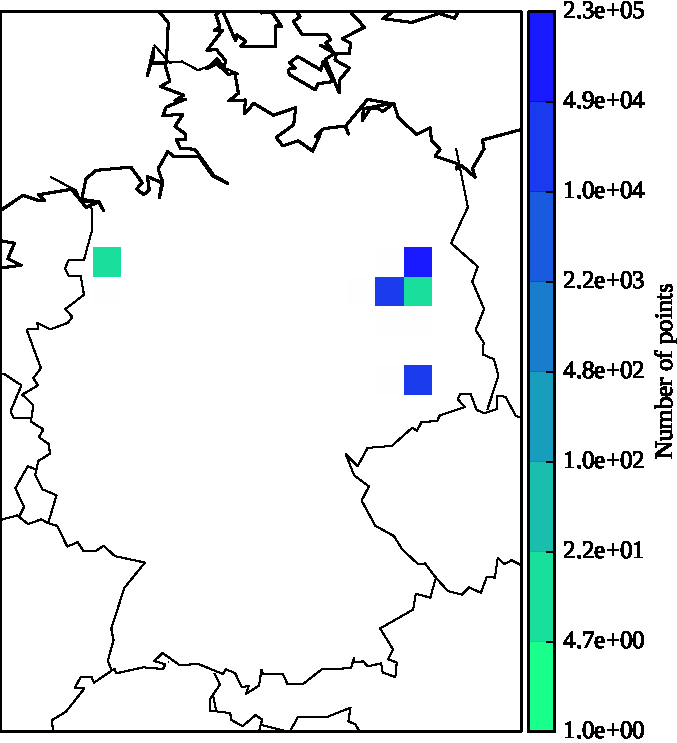
\includegraphics[width=\textwidth]{pix/freq_COM_ger_berlin.pdf}
		\caption{CM}
		%\label{fig:gull}
	\end{subfigure}
	%\,
	\begin{subfigure}[b]{.23\textwidth}
	\centering
	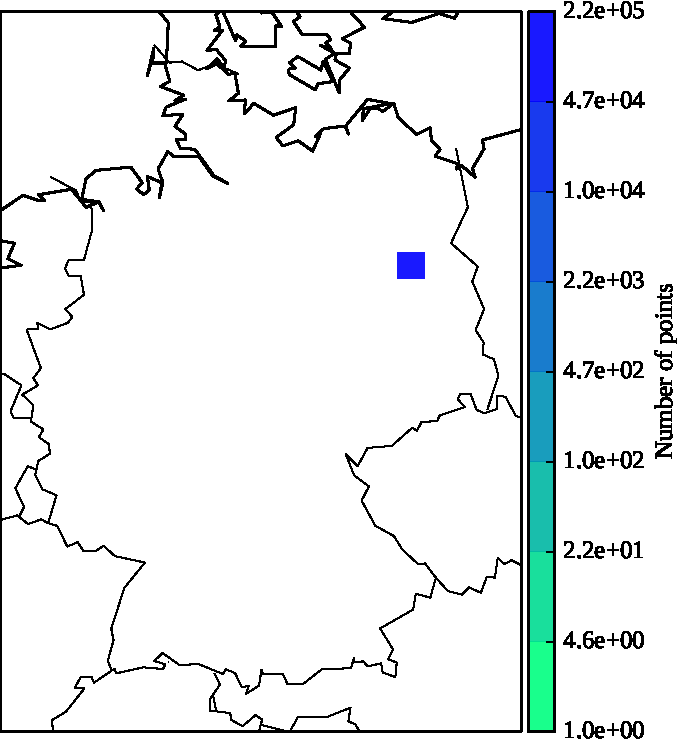
\includegraphics[width=\textwidth]{pix/freq_RW_ger_berlin.pdf}
		\caption{GM}
		%\label{fig:gull}
	\end{subfigure}
	\hfill
	\begin{subfigure}[b]{.23\textwidth}
	\centering
	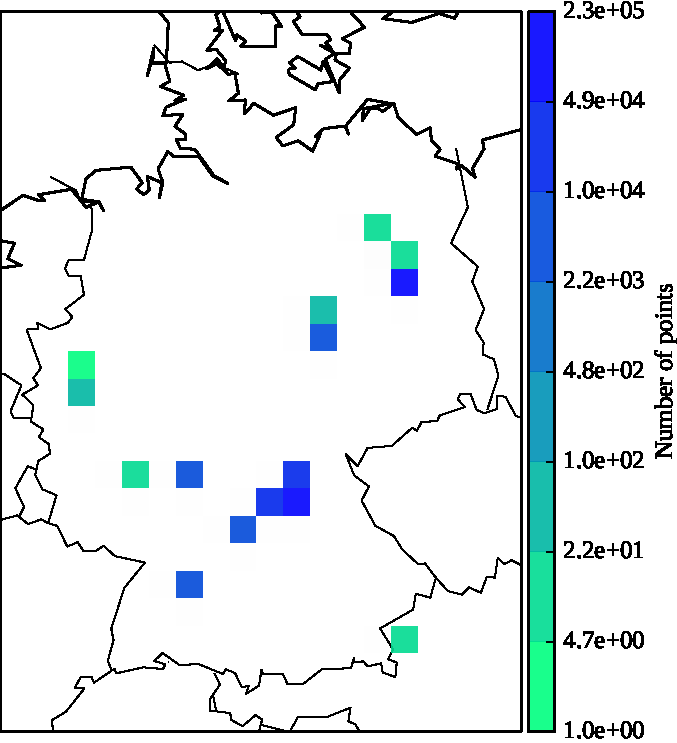
\includegraphics[width=\textwidth]{pix/freq_COM_ger_oster.pdf}
		\caption{CM}
		%\label{fig:gull}
	\end{subfigure}
	%\,
	\begin{subfigure}[b]{.23\textwidth}
	\centering
	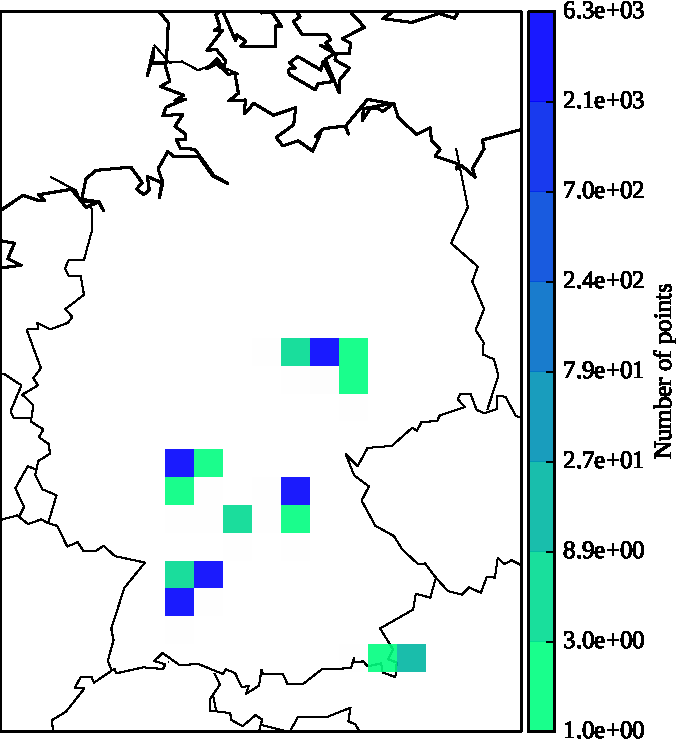
\includegraphics[width=\textwidth]{pix/freq_RW_ger_oster.pdf}
		\caption{GM}
		%\label{fig:gull}
	\end{subfigure}
	%
	\caption[Distributions for \emph{berlin}, \emph{oster} using dataset B.]{The left two distributions show $CM$ and $GM$ for \emph{berlin}, while the right pictures visualise the term \emph{oster} for dataset B.}
	\label{fig:B_comp}
\end{figure}

%                                     C USA
%
\newpage
\begin{center}
\captionof{table}{Statistics and used parameters for dataset C}
\small
\sisetup{table-parse-only}
\begin{tabular}{cSSSc}
\toprule
 & {clusters} &{clustered elements}&{noise}&{parameters}\\
\midrule
GM & 364 & 861138 & 225540&$km=300000, w_{text} = 0.1, \epsilon = 0.951$\\
CM & 343 & 1086024 & 654&$eps_{text} = 0.5, eps_{loc} = 7000$\\
\bottomrule
\end{tabular}
\end{center}
%
The last dataset C is Flickr data from the United States. The number of clusters are again very similar, but this time $GM$ has much noise, in contrast to the clusterings from dataset B. CQM scores (table~\ref{tbl:C_compare}) show a much better performance for $CM$ across the board with text and location distances alike. 
%
%
The terms used for this dataset are \emph{coast}, \emph{desert} and \emph{nature} because the same dataset as in \cite{Sengstock2012a} was used. Comparison pictures can be found in figure~\ref{fig:C_comp}. Distribution in space is similar between $GM$ and $CM$, but $CM$ has more more points in less spots, whereas $GM$ has more widespread distributions. Words describing the global region of America (\emph{unitedstates}, \emph{unitedstatesofamerica}, \emph{usa}) are unfortunately very common in all results and omitted in the further discussion.

\emph{coast} yields for $GM$ mostly cities or regions near to a coast, like \emph{houston}, \emph{california}, \emph{wortham}, \emph{sanfrancisco}, \emph{newyork} and \emph{vancuover}. General environmental terms (\emph{westcoast}, \emph{park}) appear less. Results for $CM$ are not as good, with the three top terms \emph{home45drumhillroad},\emph{elementsorganizer}, \emph{harrypotterparty} having nothing to do with a coast. Cities and environmental words are less frequent.

\enlargethispage{1\baselineskip}
\begin{table}[h]
\caption{CQM for dataset C}\label{tbl:C_compare}
\small
\centering
%\sisetup{table-parse-only}
\sisetup{table-format = 1.0(1)e2}
\begin{tabular}{cSSSS}
\toprule
Dataset & {DB} &{C}&{SW}&{D}\\
			& {\scriptsize $0<min<\infty$} &{\scriptsize $0<min<1$}&{\scriptsize $-1<max<1$}&{\scriptsize $0<max<\infty$}\\
\midrule
\multicolumn{5}{c}{Location distance}\\
\midrule
GM & 7.09e+00 & 7.01e-05 & 6.79e-01 & 2.17e-12\\
CM  & 6.96e-01 & 5.73e-07 & 8.78e-01 & 6.15e-04\\
R  & 1.29e+03 & 2.35e-01 & -1.41e-01 & 0.00e+00\\
\midrule
\multicolumn{5}{c}{Text distance}\\
\midrule
GM & 1.28e+00 & 2.70e-01 & 4.13e-01 & 0.00e+00\\
CM & 1.37e+00 & 1.42e-01 & 6.69e-01 & 0.00e+00\\
R & 3.90e+00 & 8.69e-01 & -2.05e-02 & 0.00e+00\\
\bottomrule
\end{tabular}
\end{table}

Mutual terms for \emph{desert} are \emph{nevada}, \emph{utah}, \emph{canyon} and \emph{water}, which is reasonable. $GM$ has among others more good words like \emph{mexico}, \emph{texas}, \emph{sierra},  \emph{arizona} and the global theme \emph{America} is not present. $CM$ has \emph{hike}, \emph{southwest}, \emph{desert} and \emph{rock}, but also unsuitable ones like \emph{chris} and \emph{deviatedseptum} (a common physical disorder of the nose). 

Unusual results are obtained with \emph{nature}. $CM$ shows again \emph{home45drumhillroad}, \emph{elementsorganizer}, \emph{harrypotterparty} as top results, with Microsoft Windows terms following (\emph{microsoft}, \emph{windows}, \emph{7}, \emph{skydrive}, \emph{live}) and the first \emph{nature} related term at position 26. $GM$ has more meaningful results: \emph{nature}, \emph{camping} and \emph{napavalley} are among the top ten terms, with \emph{sky}, \emph{park}, \emph{trees} and \emph{hiking} present after many different entries for \emph{tatoos} and \emph{tatto} studios.

\begin{figure}%[tbp]
	\begin{subfigure}[b]{.45\textwidth}
	\centering
	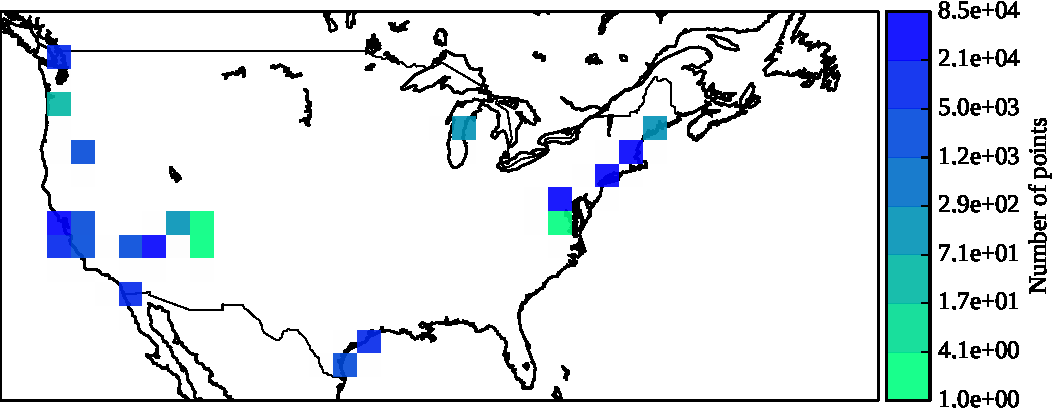
\includegraphics[width=\textwidth]{pix/freq_COM_usa_coast.pdf}
		%\caption{Frequency plot}
		%\label{fig:gull}
	\end{subfigure}
	\hfill
	\begin{subfigure}[b]{.45\textwidth}
	\centering
	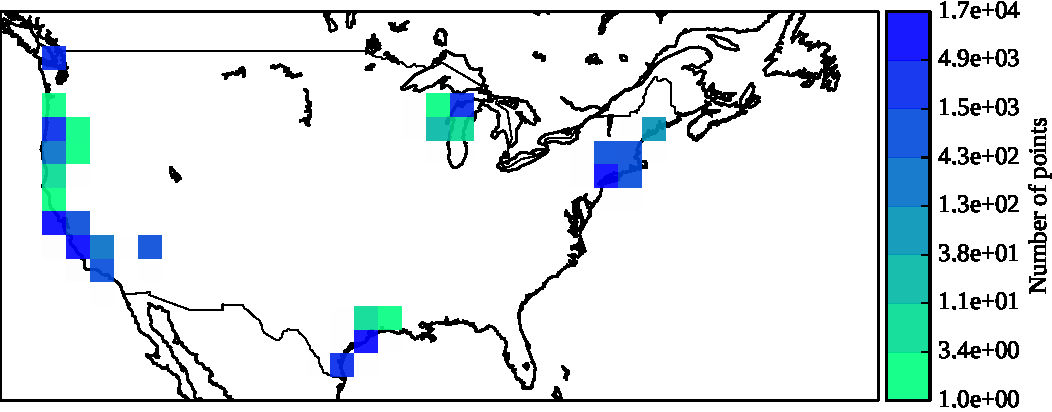
\includegraphics[width=\textwidth]{pix/freq_RW_usa_coast.pdf}
		%\caption{coast}
		%\label{fig:gull}
	\end{subfigure}
	\,
	\begin{subfigure}[b]{.45\textwidth}
	\centering
	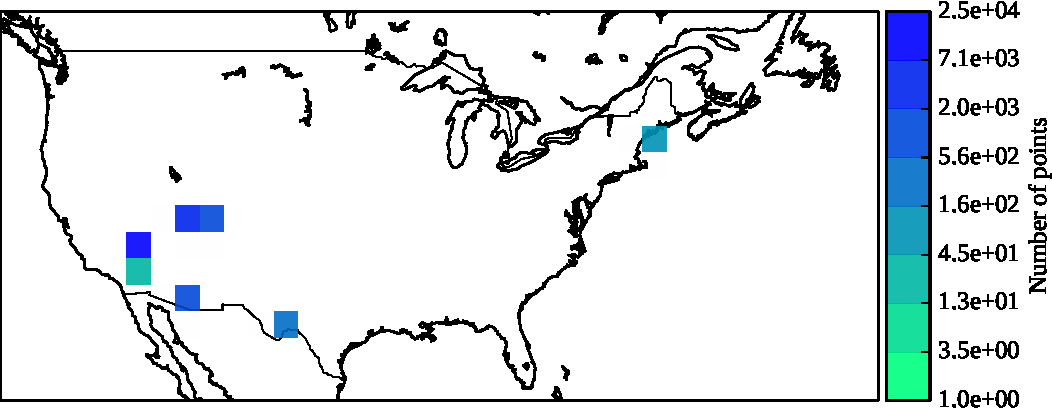
\includegraphics[width=\textwidth]{pix/freq_COM_usa_desert.pdf}
		%\caption{Frequency plot}
		%\label{fig:gull}
	\end{subfigure}
	\hfill
	\begin{subfigure}[b]{.45\textwidth}
	\centering
	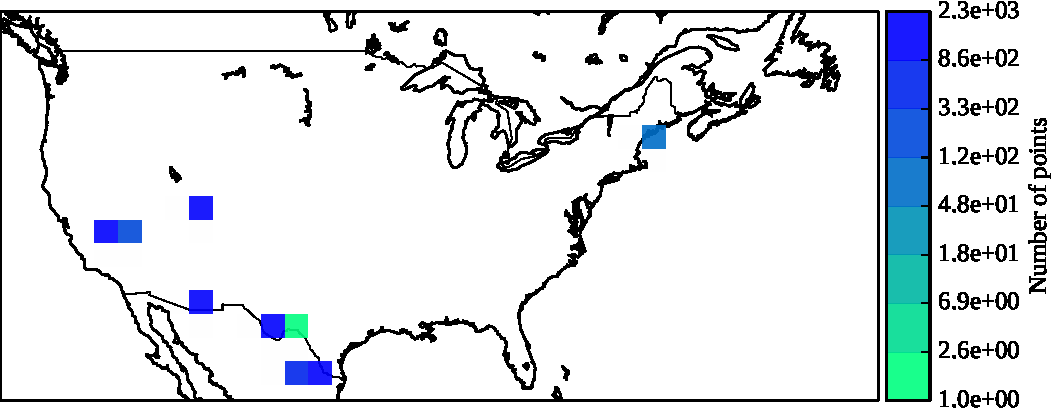
\includegraphics[width=\textwidth]{pix/freq_RW_usa_desert.pdf}
		%\caption{desert}
		%\label{fig:gull}
	\end{subfigure}
	\,
	\begin{subfigure}[b]{.45\textwidth}
	\centering
	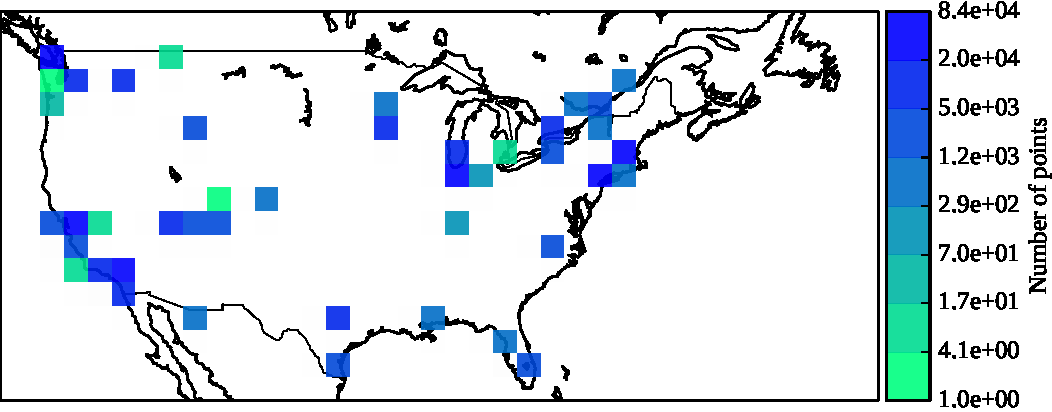
\includegraphics[width=\textwidth]{pix/freq_COM_usa_nature.pdf}
		\caption{CM}
		%\label{fig:gull}
	\end{subfigure}
	\hfill
	\begin{subfigure}[b]{.45\textwidth}
	\centering
	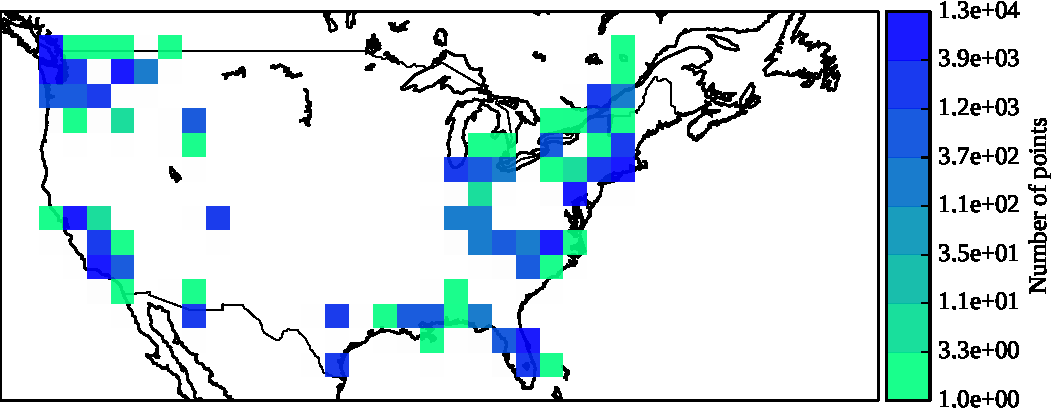
\includegraphics[width=\textwidth]{pix/freq_RW_usa_nature.pdf}
		\caption{GM}
		%\label{fig:gull}
	\end{subfigure}
	%
	\caption[Distributions for \emph{coast}, \emph{desert}, \emph{nature} with dataset C.]{The first column contains the plots for the combined metric and the second for the graph metric. The first row shows the distributions for \emph{coast}, the second for \emph{desert} and the third for \emph{nature}.}
	\label{fig:C_comp}
\end{figure}

\newpage
\noindent
$CM$ and $GM$ both deliver reasonable results, with $GM$ generally better geographic topics. Their performance is very dependent in the used dataset, as results for dataset A were poor compared to using datasets B or C.

These results were not exactly mirrored by the cluster quality measures. Compared to a random clustering, they show (some more, some less) if a clustering could generally be good. But directly comparing the scores, at least with the used basic distance functions, is not appropriate, as $CM$ usually has better scores, but $GM$ is qualitatively better. Using the jaccard distance for the CQMs resulted always in lower scores as using euclidean distance. The distance distribution with a majority of maximum distance and very few similarities seem to distort the ranges of the scores.

Despite the lack of comparability, the CQMs give generally good hints of the overall goodness of the results. Except the Dunn index ($D$) as presented in section~\ref{sec:cqm}, which in almost all cases has the same score of $0.0$, which leads to the assumption that real world cases have clusters in very near proximity more often than less. The Davies-Bouldin ($DB$) and $C$ indices fare quite well, but comparisons are always about the order of magnitude, and results are less constant in their representably of how well a result truly is. Silhouette width ($SW$) generates meaningful scores, which are easy to comprehend and correspond usually quite well to the observed characteristics of the clusterings.

\chapter{Summary and future work}\label{chap:future}
%\emph{%
%This final chapter gives a short overview about what has been shown in this thesis, and which topics and work c
%}

%\section{Summary}
%own contributions, was wurde gezeigt

In summery, two different distance metrics were implemented, and used with the cluster algorithm DBSCAN to extract geographical topics from big real world datasets. The first distance metric was a naive vector based approach with a combined distance based on an euclidean distance on GPS data, and a jaccard distance based on text data. The second distance metric was based on random walks on graphs. Base graphs were generated with Delaunay triangulations based on the GPS data, and augmented edges and nodes were added based on the text data. Qualitative evaluation showed, that both methods can give reasonable results, if the used dataset is suited. The graph based distance metric performed overall better than the vector based approach.

Quantitative evaluation was conducted with four cluster evaluation measures based on basic distance measures between location and text, in order to reveal their usefulness in comparing different geographical topic results and in indicating the general goodness of the overall clustering results. Quantitative evaluation with datasets that big is usually not done. The best results were delivered by the measure Silhouette width, with very good indications of good clusterings. But performing meaningful comparisons without qualitative evaluation is not possible with this setup. Nonetheless $SW$ with these basic distances is a useful tool in filtering the bad results, and leave the good ones for further subjective investigation.

%\section{Future work}
Which leads to different possibles for future work.
\begin{description}
\item[Graph distance] More attributes can be used, like timestamps or user ids. The graph distance is very flexible regarding such extensions. General idea behind this is, that a user is more likely to write about a few topics, which would group them even more. The same applies to timestamps.

Another idea is to connect the augmented nodes in order to get higher probabilities among attributes often used together. But this would require to remove certain edges between structural and augmented nodes to have no double connections through the same attributes.

\item[Cluster Quality measures] Silhouette width is a good basis, and other distance functions could result in results more comparable. Considering landmarks or regional topics, different distance functions could be used to evaluate different aspects of the topics. Basic euclidean for landmarks and events, and other functions which promote other nodes at certain distances and punish nodes which are near for regional or global topics.

Different functions for comparing text should be useful as well, which leads to the next work idea.

\item[Datasets] The difference between the performances in topic generation using dataset A to B and C was quite big. The only preprocessing of the datasets was the removal of common stop words. Results show many, essentially same words listed individually. Performing more preprocessing to align words (by reducing plurals for example) or splitting composited words could result in better results or could enable other distance functions.
\end{description}
%
Usage of the geographic topic discovery as described in this thesis for real world scenarios is unlikely given better qualitative results \cite{Sengstock2012a, Yin2011, Hong2012}. But using Silhouette width seems to be viable for general evaluation of geographic topic algorithms.

% !TeX program = lualatex
% !TeX root = main.tex
\appendix
\chapter{Appendix}\label{chap:appendix}
%\enlargethispage*{100\baselineskip}
%\begin{table}[h!]
%\footnotesize
%\caption{Four random walks with different lengths based on figure~\ref{fig:graph_for_examples}, all starting at node 0. First column marks the node, second column all path leading to this node, and the third column calculates the individual path probabilities and sums them all up.}\label{tbl:RW}

%\noindent\begin{minipage}{\textwidth}
    \centering
    \captionof{table}[Random walks with paths]{Four random walks with different lengths based on figure~\ref{fig:graph_for_examples}, all starting at node 0. First column marks the node, second column all path leading to this node, and the third column calculates the individual path probabilities and sums them all up.}\label{tbl:RW}
\footnotesize
\begin{multicols}{2}
\begin{tabular}{lcr}
\toprule
\multicolumn{2}{c}{l = 1}&\phantom{$1.0 \cdot 0.33 \cdot 0.5 \cdot 0.33$}\\
\midrule
0	&						&$=0.0$\\
\hline
1	&				 		&$=0.0$\\
\hline
2	&					 	&$=0.0$\\
\hline
\multirow{2}{*}{3}&0-3				 	&$1.0$\\
	&\phantom{0-3-2-3-2}						&$=1.0$\\
\bottomrule
\end{tabular}

\vspace*{1em}

\begin{tabular}{lcr}
\toprule
\multicolumn{2}{c}{l = 2}&\phantom{$1.0 \cdot 0.33 \cdot 0.5 \cdot 0.33$}\\\midrule
\multirow{2}{*}{0}&0-3-0			&$1.0 \cdot 0.33$\\
	&					&$=0.33$\\
\hline
\multirow{2}{*}{1}&0-3-1	 		&$1.0 \cdot 0.33$\\
	&					&$=0.33$\\
\hline
\multirow{2}{*}{2}&0-3-2		 	&$1.0 \cdot 0.33$\\
	&					&$=0.33$\\
\hline
3	&\phantom{0-3-2-3-2}					 &$=0.0$\\
\bottomrule
\end{tabular}

\vspace*{1em}

\begin{tabular}{lcr}
\toprule
\multicolumn{2}{c}{l = 3}&\phantom{$1.0 \cdot 0.33 \cdot 0.5 \cdot 0.33$}\\\midrule
0	&						&$=0.0$\\
\hline
\multirow{2}{*}{1}&0-3-2-1 			&$1.0 \cdot 0.33 \cdot 0.5$\\
	&						&$=0.165$\\
\hline
\multirow{2}{*}{2}&0-3-1-2 			&$1.0 \cdot 0.33 \cdot 0.5$\\
	&						&$=0.165$\\
\hline
\multirow{4}{*}{3}&0-3-0-3 			&$1.0 \cdot 0.33 \cdot 1.0$\\
	&0-3-1-3 			&$1.0 \cdot 0.33 \cdot 0.5$\\
	&0-3-2-3 			&$1.0 \cdot 0.33 \cdot 0.5$\\
	&\phantom{0-3-2-3-2}&$=0.66$\\
\bottomrule
\end{tabular}

%\vspace*{1em}

\begin{tabular}{lcr}
\toprule
\multicolumn{2}{c}{l = 4}&\phantom{$1.0 \cdot 0.33 \cdot 0.5 \cdot 0.33$}\\\midrule
\multirow{4}{*}{0}&0-3-0-3-0	&$1.0 \cdot 0.33 \cdot 1.0 \cdot 0.33$\\
	&0-3-1-3-0	&$1.0 \cdot 0.33 \cdot 0.5 \cdot 0.33$\\
	&0-3-2-3-0	&$1.0 \cdot 0.33 \cdot 0.5 \cdot 0.33$\\
	&					&$=0.22$\\
\hline
\multirow{5}{*}{1}&0-3-1-2-1	&$1.0 \cdot 0.33 \cdot 0.5 \cdot 0.5$\\
	&0-3-0-3-1	&$1.0 \cdot 0.33 \cdot 1.0 \cdot 0.33$\\
	&0-3-1-3-1	&$1.0 \cdot 0.33 \cdot 0.5 \cdot 0.33$\\
	&0-3-2-3-1	&$1.0 \cdot 0.33 \cdot 0.5 \cdot 0.33$\\
	&					&$=0.31$\\
\hline
\multirow{5}{*}{2}&0-3-2-1-2	&$1.0 \cdot 0.33 \cdot 0.5 \cdot 0.5$\\
	&0-3-0-3-2	&$1.0 \cdot 0.33 \cdot 1.0 \cdot 0.33$\\
	&0-3-1-3-2	&$1.0 \cdot 0.33 \cdot 0.5 \cdot 0.33$\\
	&0-3-2-3-2	&$1.0 \cdot 0.33 \cdot 0.5 \cdot 0.33$\\
	&					&$=0.31$\\
\hline
\multirow{3}{*}{3}&0-3-2-1-3	&$1.0 \cdot 0.33 \cdot 0.5 \cdot 0.5$\\
	&0-3-1-2-3	&$1.0 \cdot 0.33 \cdot 0.5 \cdot 0.5$\\
	&					&$=0.16$\\
\bottomrule
\end{tabular}
\end{multicols}
%\end{table}
%\end{minipage}

%\begin{table}%[h]
%\caption{Five random walks with different lengths based on figure~\ref{fig:graph_for_examples} with transition matrix $P$.}\label{tbl:RW2}

%\noindent\begin{minipage}{\textwidth}
\centering
\normalsize
\captionof{table}[Random wlks with transition matrix.]{Five random walks with different lengths based on figure~\ref{fig:graph_for_examples} with transition matrix $P$.}\label{tbl:RW2}
\begin{multicols}{2}
\centering
$l = 1 \equiv P^1$
\vspace{-.5em}
\[
\begin{pmatrix*}[S]
0.0	& 0.0	& 0.0	& 1.0\\
0.0	& 0.0	& 0.5	& 0.5\\
0.0	& 0.5	& 0.0	&0.5\\
0.333	& 0.333	& 0.333	&0.0\text{\phantom{$00$}}
\end{pmatrix*}
\]\\
%\vspace{1.em}

$l = 2 \equiv P^2$
\vspace{-.5em}
\[
\begin{pmatrix*}[S]
0.333	& 0.333	& 0.333	& 0.0\\
0.167	& 0.416	& 0.167	& 0.25\\
0.167	& 0.167	& 0.415	& 0.25\\
0.0	& 0.167	& 0.167	& 0.667
\end{pmatrix*}
\]\\

$l = 3 \equiv P^3$
\vspace{-.5em}
\[
\begin{pmatrix*}[S]
0.0	    & 0.167	& 0.167	& 0.666\\
0.083	& 0.167	& 0.292	& 0.458\\
0.083	& 0.292	& 0.167	& 0.458\\
0.222	& 0.306	& 0.306	& 0.166
\end{pmatrix*}
\]\\

%\vspace{1.em}
$l = 4 \equiv P^4$
\vspace{-.5em}
\[
\begin{pmatrix*}[S]
0.222	& 0.306	& 0.306	& 0.166\\
0.153	& 0.298	& 0.236	& 0.312\\
0.153	& 0.236	& 0.298	& 0.312\\
0.056	& 0.208	& 0.208	& 0.528
\end{pmatrix*}
\]\\

%\vspace{1.em}
$n \rightarrow \infty, l = n \equiv P^n$
\vspace{-.5em}
\[
\begin{pmatrix*}[S]
0.125	& 0.250	& 0.250	& 0.375\\
0.125	& 0.250	& 0.250	& 0.375\\
0.125	& 0.250	& 0.250	& 0.375\\
0.125	& 0.250	& 0.250	& 0.375
\end{pmatrix*}
\]\\

%%%%%PHANTOM%%%%%%%%
\phantom{
$n \rightarrow \infty, l = n \equiv P$
$\begin{pmatrix*}[S]
0.125	& 0.250	& 0.250	& 0.375\\
0.125	& 0.250	& 0.250	& 0.375\\
0.125	& 0.250	& 0.250	& 0.375\\
0.125	& 0.250	& 0.250	& 0.375
\end{pmatrix*}$}
\end{multicols}
%\end{table}
%\end{minipage}

\newpage
\centering
\normalsize
%\begin{table}%[h]
\captionof{table}[Random walk distances]{Distances between nodes with the random walk model based on figure~\ref{fig:graph_for_examples}.}\label{tbl:RW3}
\begin{multicols}{2}
\centering
%c = 0.1
$l = 1$
\vspace{-.5em}
\[
\begin{pmatrix*}[S]
0.0	& 0.0	& 0.0	& 0.09\\
0.0	& 0.0	& 0.045	& 0.045\\
0.0	& 0.045	& 0.0	& 0.045\\
0.030	& 0.030	& 0.030	& 0.0
\end{pmatrix*}
\]\\

$l = 2$
\vspace{-.5em}
\[
\begin{pmatrix*}[S]
0.027	& 0.027	& 0.027	& 0.090\\
0.013	& 0.034	& 0.058	& 0.065\\
0.014	& 0.058	& 0.034	& 0.065\\
0.030	& 0.043	& 0.043	& 0.054
\end{pmatrix*}
\]\\

$l = 3$
\vspace{-.5em}
\[
\begin{pmatrix*}[S]
0.027	& 0.039	& 0.039	& 0.139\\
0.020	& 0.046	& 0.080	& 0.099\\
0.020	& 0.080	& 0.046	& 0.099\\
0.046	& 0.066	& 0.066	& 0.066
\end{pmatrix*}
\]\\

$l = 4$
\vspace{-.5em}
\[
\begin{pmatrix*}[S]
0.042	& 0.059	& 0.059	& 0.150\\
0.030	& 0.065	& 0.095	& 0.119\\
0.030	& 0.095	& 0.065	& 0.119\\
0.050	& 0.079	& 0.079	& 0.101
\end{pmatrix*}
\]\\

$l = 4, mean distances$
\vspace{-.5em}
\[
\begin{pmatrix*}[S]
0.042	& 0.044	& 0.044	& 0.100\\
0.044	& 0.065	& 0.095	& 0.099\\
0.044	& 0.095	& 0.065	& 0.099\\
0.100	& 0.099	& 0.099	& 0.101
\end{pmatrix*}
\]\\

\phantom{
$\begin{pmatrix*}[S]
0.042	& 0.044	& 0.044	& 0.100\\
0.044	& 0.065	& 0.095	& 0.099\\
0.044	& 0.095	& 0.065	& 0.099\\
0.100	& 0.099	& 0.099	& 0.101
\end{pmatrix*}$}
\end{multicols}
%\end{table}


%\begin{table}[htb]
\newpage
\centering
\sisetup{table-parse-only}
\captionof{table}{Dataset A acakfilm}%\label{tbl:top_words}
\begin{tabular}{cScS}
\toprule
\multicolumn{2}{c}{GM}&\multicolumn{2}{c}{CM}\\
\midrule
acakfilm  & 4086  & acakfilm  & 4086\\
muzejninoc &  23 & gfprague  & 83\\
photo  & 3  & muzejninoc  & 64\\
prague  & 2 & groupama  & 34\\
1 &  2 & fb  & 18\\
muzejni  & 2 & prague  & 14\\
9 &  2 & photo  & 10\\
fb  & 2 & stavka  & 9\\
12 &  2 & fail  & 9\\
fx  & 1 & sunrise  & 9\\
stojitozapicu  & 1 & sunset  & 9\\
wp7  & 1  & anana  & 8\\
torah  & 1 & kazmarytmus  & 8\\
gotdressedinthedark & 1 & praha  & 7\\
praha  & 1  & 3  & 6\\
fail  & 1  & genesyslab  & 5\\
forex &  1 & eurogang11  & 5\\
nebrat &  1  & revizori  & 4\\
skola  & 1 & ee  & 4\\
travel  & 1  & 1  & 4\\
sovereign  & 1 & 4  & 3\\
3  & 1 & winning  & 3\\
kokoti  & 1 & cctr  & 3\\
yuanli  & 1 & foto  & 3\\
hardrockcafe  & 1 & museum  & 3\\
\bottomrule
\end{tabular}
%\end{table}



%\begin{table}[htb]
\newpage
\centering
\sisetup{table-parse-only}
\captionof{table}{Dataset A brandenburg}%\label{tbl:top_words}
\begin{tabular}{cScS}
\toprule
\multicolumn{2}{c}{GM}&\multicolumn{2}{c}{CM}\\
\midrule
nowplaying & 2448  & nowplaying  & 4359\\
ger &  1000  & ger  & 1656 \\
brandenburg  & 959  & brandenburg  & 1106 \\
bbradio  & 656  & bbradio  & 656 \\
iphone  & 231  & stream  & 261 \\
stream  & 180  & iphone  & 231 \\
rocks  & 162  & kassel  & 222\\
hits  & 149  & berlin  & 211\\
berlin  & 142  & schwerin  & 209 \\
showopenerstingervollm  & 118  & facebook  & 184 \\
app  & 113  & rocks  & 162 \\
fb  & 87 & hits  & 149\\
oranienburg  & 86 & radioteddy  & 146\\
wittenberge  & 79  & radio  & 143\\
rihanna  & 76  & potsdam  & 143\\
pritzwalk  & 76 & hessen  & 133\\
katyperry  & 75  & katyperry  & 125\\
potsdam  & 75  & showopenerstingervollm  & 118\\
huette  & 74 & app  & 113\\
ladygaga  & 73 & ladygaga  & 112\\
wittstock  & 66  & taiocruz  & 96\\
frankfurtoder  & 64 & brunomars  & 96\\
ffo  & 64  & rihanna  & 89\\
perleberg  & 63  & fb  & 87\\
radio  & 62 & oranienburg  & 86\\
\bottomrule
\end{tabular}
%\end{table}



%\begin{table}[htb]
\newpage
\centering
\sisetup{table-parse-only}
\captionof{table}{Dataset A berlin}%\label{tbl:top_words}
\begin{tabular}{cScS}
\toprule
\multicolumn{2}{c}{GM}&\multicolumn{2}{c}{CM}\\
\midrule
nowplaying  & 2457  & nowplaying  & 4405 \\
ger  & 1008  & ger &  1664\\
brandenburg  & 959  & brandenburg  & 1106\\
bbradio & 656  & bbradio  & 656\\
berlin  & 286  & berlin  & 430\\
iphone &  238  & duendari  & 348\\
stream  & 180  & news  & 276\\
rocks  & 162 & stream  & 261\\
hits &  149  & iphone &  248\\
fb  & 118 & fb  & 248\\
showopenerstingervollm  & 118  & kassel  & 222\\
app  & 114  & schwerin  & 209\\
tcbnk  & 96  & facebook  & 198\\
oranienburg  & 86 & bibtag11  & 171\\
wittenberge  & 79  & rocks  & 162 \\
rihanna &  76 & hits &  149\\
pritzwalk  & 76  & radioteddy  & 146\\
potsdam  & 75  & radio  & 144\\
ladygaga  & 75  & potsdam  & 143\\
katyperry  & 75  & hessen  & 133\\
huette &  74  & katyperry  & 125\\
wittstock &  66  & hamburg  & 122\\
ffo  & 64 & showopenerstingervollm  & 118\\
frankfurtoder  & 64 & ladygaga  & 117\\
perleberg  & 63 & app & 114\\
\bottomrule
\end{tabular}
%\end{table}



%\begin{table}[htb]
\newpage
\centering
\sisetup{table-parse-only}
\captionof{table}{Dataset A stuttgart}%\label{tbl:top_words}
\begin{tabular}{cScS}
\toprule
\multicolumn{2}{c}{GM}&\multicolumn{2}{c}{CM}\\
\midrule
stuttgart  & 55 & s21  & 86\\
jobs &  32  & stuttgart &  59\\
fehmarn  & 31  & fb & 58 \\
job  & 27  & jobs  & 47\\
turkeywantsgaga  & 27  & frankfurt  & 47 \\
alstomjobs  & 27  & gwm  & 45\\
tweetmyjobs  & 23  & baustop &  34\\
djht  & 20  & hessentag  & 31 \\
s21  & 14  & turkeywantsgaga  & 30\\
domian  & 10  & alstomjobs  & 27 \\
smcst &  9  & job  & 27\\
pforzheim  & 9  & blockade  & 23\\
gntmf  & 9  & tweetmyjobs  & 23\\
npbs  & 7  & intersolar  & 18 \\
wm  & 7  & devconnections  & 17\\
frauenfussball  &  7 & polizei  & 17\\
ferienjob  & 7  & aussitzen  & 14 \\
businessmgmt  & 7  & endomondo  & 12\\
ios5  & 6  & ferienjob & 12\\
gid  & 6  & projektaus  & 11 \\
stuttgarternachr  & 5  & ios5  & 11\\
daimlerag  & 5  & immo  & 10 \\
ibmdeutschlandgmbh  & 4  & smcst  & 10 \\
renningen  & 4  & domian  & 10\\
kde  & 4  & gntmf  & 10\\
\bottomrule
\end{tabular}
%\end{table}



%\begin{table}[htb]
\newpage
\centering
\sisetup{table-parse-only}
\captionof{table}{Dataset A hamburg}%\label{tbl:top_words}
\begin{tabular}{cScS}
\toprule
\multicolumn{2}{c}{GM}&\multicolumn{2}{c}{CM}\\
\midrule
hamburg &  82 & hamburg  & 129\\
fb  & 22  & twexit  & 86\\
obs  & 20  & fb  & 49\\
fh3  & 18 & groningen  & 39\\
leadawards  & 14 & f1  & 37\\
ff  & 12 & tadaa  & 37\\
jobs  & 10 & np  & 28 \\
stellenangebot  & 10 & wirsounterwegs &  27\\
grunerjahrstern  & 8 & fh3  & 26\\
demo  & 7 & fail  & 26 \\
oldenburg  & 6 & demo &  25\\
thanksjustin  & 6 & degene  & 20\\
esgehtrunter  & 5 & cms11  & 18 \\
fail  & 5 & endomondo  & 17\\
wirsounterwegs &  5 & pp11  & 17\\
engardemarketinggmbh  & 5 & leadawards  & 16\\
echofon &  5 & jobs  & 16\\
mehrunihh  & 4 & twexitttttt  & 15\\
job  & 4 & durftevragen  & 14\\
unserhamburgunsernetz  & 4 & eurovoetbal  & 14 \\
dmwhh & 4 & kiel  & 13\\
location  & 4 & salut &  12\\
twitter &  4  & in  & 12\\
nowplaying  & 4  & bremen  & 12\\
ios5  & 4  & cams21 & 11\\
\bottomrule
\end{tabular}
%\end{table}




%\begin{table}[htb]
\newpage
\centering
\sisetup{table-parse-only}
\captionof{table}{Dataset B berlin}%\label{tbl:top_words}
\begin{tabular}{cScS}
\toprule
\multicolumn{2}{c}{GM}&\multicolumn{2}{c}{CM}\\
\midrule
facebook  & 61629  & facebook  & 65563\\
metros  & 43279  & metros  & 51151\\
trains  & 41724 & trains  & 41724 \\
lrt &  23607 & lrt &  35406 \\
berlin &  23359  & berlin  & 24836 \\
stations  & 22738  & stations &  22738\\
bus  & 15742  & dresden  & 17922 \\
architecture  & 11809  & bus  & 15743 \\
wayfinding  & 11807  & wayfinding  & 15740 \\
holocaustmemorial  & 8849  & architecture  & 11822 \\
planes  & 7171  & deutschland  & 11766\\
friends  & 6991  & germany  & 10197 \\
wctoilet  & 6546  & holocaustmemorial  & 8849 \\
honecker  & 6497  & planes  & 7171\\
kissing &  6497 & friends  & 6991 \\
leonid &  6497  & stadtschloss  & 6643\\
brezhnev  & 6497  & brühlscheterrassen  & 6643\\
erich  & 6497  & wctoilet &  6546\\
sanssouci  & 5934  & kissing  & 6498 \\
deutschland  & 5812 & honecker  & 6497 \\
mygearandme &  5805  & leonid  & 6497 \\
germany  & 4207  & brezhnev  & 6497 \\
europe  & 4184  & erich  & 6497 \\
berlinerdom  & 4171 & sanssouci  & 5934 \\
abend  & 4168 & mygearandme  & 5805 \\
\bottomrule
\end{tabular}
%\end{table}



%\begin{table}[htb]
\newpage
\centering
\sisetup{table-parse-only}
\captionof{table}{Dataset B oster}%\label{tbl:top_words}
\begin{tabular}{cScS}
\toprule
\multicolumn{2}{c}{GM}&\multicolumn{2}{c}{CM}\\
\midrule
dekoration  & 6258  & ostern  & 178653 \\
brauch &  6258  & osterbrunnentour  & 178652\\
easter  & 6258  & easter  & 178652 \\
decoration &  6258  & osterei  & 156294 \\
ostern &  6258  & easteregg  & 156294 \\
tradition &  6258  & ei  & 156294 \\
egg  & 6258  & tradition  & 156294 \\
ei  & 6258  & dekoration  & 156294\\
custom  & 6258 & egg  & 156294 \\
osterbrunnentour  & 6258 & decoration &  156294\\
osterei  & 6258  & custom  & 156294 \\
easteregg  & 6258  & brauch &  156294 \\
mansfelderberwerksbahn  & 6141  & facebook  & 65562\\
boksthal  & 6141  & metros  & 51151 \\
ok &  6141  & trains  & 41724 \\
orensteinkoppel  & 6141 & lrt  & 23607\\
klostermansfeld &  6141  & stations  & 22738 \\
mirrorsphere  & 3863  & berlin  & 21865 \\
kugelkurve &  3863  & deutschland  & 18045\\
symmetrie &  3863  & germany  & 16570 \\
münchhausen  & 3863  & bus  & 15743 \\
steinkugeln  & 3863  & photo  & 12141 \\
sphere  & 3863  & foto  & 12140 \\
kugelspiegelung  & 3863  & fotografie  & 12140\\
kugeln &  3863 & fotos & 12140\\
\bottomrule
\end{tabular}
%\end{table}




%\begin{table}[htb]
\newpage
\centering
\sisetup{table-parse-only}
\captionof{table}{Dataset C coast}%\label{tbl:top_words}
\begin{tabular}{cScS}
\toprule
\multicolumn{2}{c}{GM}&\multicolumn{2}{c}{CM}\\
\midrule
houston  & 15783  & home45drumhillroad &  67314 \\
california  & 10891  & elementsorganizer  & 67314 \\
usa &  9565 1 & harrypotterparty  & 67035 \\
wortham  & 7118  & usa  & 50727\\
center &  7118  & unitedstates  & 42718\\
sanfrancisco  & 5870  & california  & 39286 \\
unitedstates  & 5453  & border  & 35550 \\
unitedstatesofamerica  & 4440  & pjenniferlongmire  & 29928 \\
westcoast  & 4362  & nj &  25961\\
park  & 4097  & newjersey  & 25765\\
texas  & 4017  & post  & 25493\\
america  & 3751  & nrhp  & 25330\\
trip &  3746  & nationalhistoriclandmark &  25330\\
travel  & 3457  & nationalregister & 25327 \\
birthday  & 3410  & nhl  & 25327\\
175  & 3410 & historic  & 25327\\
market  & 3410  & army  & 25326 \\
square  & 3410  & nationalparkservice  & 25326\\
costume  & 3056  & fort  & 25325 \\
newyork  & 2981  & sandyhook  & 25325\\
canada  & 2845  & officersquarters  & 25325\\
vancuover  & 2841  & gatewaynationalrecreationarea  & 25325\\
cityscapes  & 2841  & nps &  25325\\
birdblind  & 2837  & historicdistrict  & 25325\\
marsh  & 2837  & forthancock  & 25325\\
\bottomrule
\end{tabular}
%\end{table}




%\begin{table}[htb]
\newpage
\centering
\sisetup{table-parse-only}
\captionof{table}{Dataset C desert}%\label{tbl:top_words}
\begin{tabular}{cScS}
\toprule
\multicolumn{2}{c}{GM}&\multicolumn{2}{c}{CM}\\
\midrule
canyon  & 2845 & nevada  & 16588\\
park  & 2759 & lasvegas  & 15605\\
mexico  & 2522 & travel  & 11068\\
landscape  & 2464 & vegas  & 6718\\
california  & 2354 & deviatedseptum  & 6364\\
texas  & 2262 & chris  & 6364\\
bigbend  & 2261 & unitedstates  & 6354\\
westtexas  & 2259 & usa  & 6267\\
nevada  & 2161 & unitedstatesofamerica  & 5608\\
sierra  & 2161 & clarkcounty &  5504\\
national  & 2161 & utah  & 4381\\
kings  & 2161 & hike  & 3419\\
river  & 2037 & neon  & 3396\\
monterrey  & 1809 & southwest  & 3372\\
lake  & 1780 & canyon  & 3181\\
water  & 1656 & water &  3150\\
utah  & 1632 & formations  & 3136\\
moab  & 1630 & desert  & 3126\\
arizona  & 1239 & landscape  & 3119\\
2011  & 1214 & nature  & 3073\\
nuevoleon  & 1214 & outdoors  & 3066\\
macroplaza  & 1214 & fremontst  & 2894\\
meadow  & 1092 & rock  & 2496\\
san  & 1092 & coloradoplateau  & 2432\\
evolution  & 1092 & kanecounty  & 2430\\
\bottomrule
\end{tabular}
%\end{table}

%\begin{table}[htb]
\newpage
\centering
\sisetup{table-parse-only}
\captionof{table}{Dataset C nature}%\label{tbl:top_words}
\begin{tabular}{cScS}
\toprule
\multicolumn{2}{c}{GM}&\multicolumn{2}{c}{CM}\\
\midrule
unitedstates & 37384  & unitedstates & 67585\\
nature  & 25504  & elementsorganizer  & 67338\\
northamerica  & 18644  & home45drumhillroad  & 67314\\
camping  & 17318  & harrypotterparty  & 67035\\
usa  & 14101  & usa  & 62048\\
napavalley  & 9226  & california  & 45275\\
washington  & 9170  & live  & 31897\\
tattoos  & 9166  & windows  & 31893\\
napavalleycalifornia  & 9166  & skydrive20110926backup  & 31891\\
flyingcolorstattoo  & 9166  & 20110926  & 31891\\
hiking  & 9165  & lowry  & 31891\\
californiatattoos  & 9165  & microsoft  & 31891\\
tattooedwomen  & 9165  & serenity  & 31891\\
tatto  & 9164  & antonio  & 31891\\
trees  & 9164  & edward  & 31891\\
tatoo  & 9164  & phone &  31891\\
pennsylvaniastateparks  & 9131  & focus  & 31891\\
water  & 9131  & backup  & 31891\\
canada  & 8566  & labanex  & 31891\\
tatoos  & 8391  & 7  & 31891\\
winecountrytattoo  & 7444  & anthony  & 31891\\
fctattoonapa  & 7443  & alyanna  & 31891\\
shishibeach  & 6554  & skydrive  & 31891\\
park  & 5180  & samsung  & 31891\\
sky  & 4380 & pjenniferlongmire  & 29928\\
\bottomrule
\end{tabular}
%\end{table}

%\chapter{Introduction}
%\section{Spatial data}
%\subsection{Graph representation}

%\chapter{Algorithms}

%\chapter{Implementation}

%\chapter{Evaluation}

%\chapter{Summary}

%\chapter{Appendix}






% References (Literaturverzeichnis):
% a) Style (with abbreviations: use alpha):
%\bibliographystyle{unsrt}
% b) The File:
%\bibliography{library.bib}
\printbibliography

\end{document}
